\documentclass[a4paper, 11pt]{article}

\usepackage{amsmath,amsfonts,amssymb,amsthm,graphicx,graphics,epsf}
\setcounter{tocdepth}{3}
\usepackage{graphicx}

\usepackage{algorithmic}
\usepackage{algorithm}
\usepackage{hyperref,color}
%\usepackage{comment}
%\usepackage{url}
\usepackage{xspace}
%\usepackage{lineno}
%\graphicspath{{img/}} % No need to write this for every figure
%\linenumbers


\usepackage{geometry}

\newcommand{\etal}{\emph{et al}}

\newtheorem{theorem}{Theorem}[section]
\newtheorem{corollary}[theorem]{Corollary}
\newtheorem{lemma}[theorem]{Lemma}
\newtheorem{proposition}[theorem]{Proposition}
\newtheorem{observation}[theorem]{Observation}
\newtheorem{problem}[theorem]{Problem}
\newtheorem{definition}[theorem]{Definition}
\newtheorem{conjecture}[theorem]{Conjecture}
\newtheorem{question}[theorem]{Question}



%%
%% Here you may place your macros using \newcommand{}{}
%%


  
  \newcommand{\red}[1]{{\color{red} #1}}
  
  \newcommand{\ch}[1]{\ensuremath{\textsc{ch}(#1)}}


\begin{document}



\title{Compatible Connectivity-Augmentation \\ of Disconnected Graphs}





\author{Second Bellairs Workshop on Geometry and Graphs}
\date{}

\maketitle
\begin{abstract}

\end{abstract}


%A category including the fourth, optional field follows..

\section{Introduction}

We consider the following problem, which will be more carefully formalized
below.  We are given several different planar straight-line drawings
of the same graph, $\mathcal G$, which is not connected.
We wish to make $\mathcal G$ connected by adding vertices and edges in
such a way that these vertices and edges can also be added to the planar
straight-line drawings of $\mathcal G$ while preserving the planarity of
the drawings.  The objective is to do this while minimizing the number
of edges and vertices added.  As the example in Figure~\ref{fig:bad-example} shows, it is not always possible to just add edges to $\mathcal G$; sometimes additional vertices are necessary.

\begin{figure}
  \centering{
    \begin{tabular}{c@{\hspace{2cm}}c}
      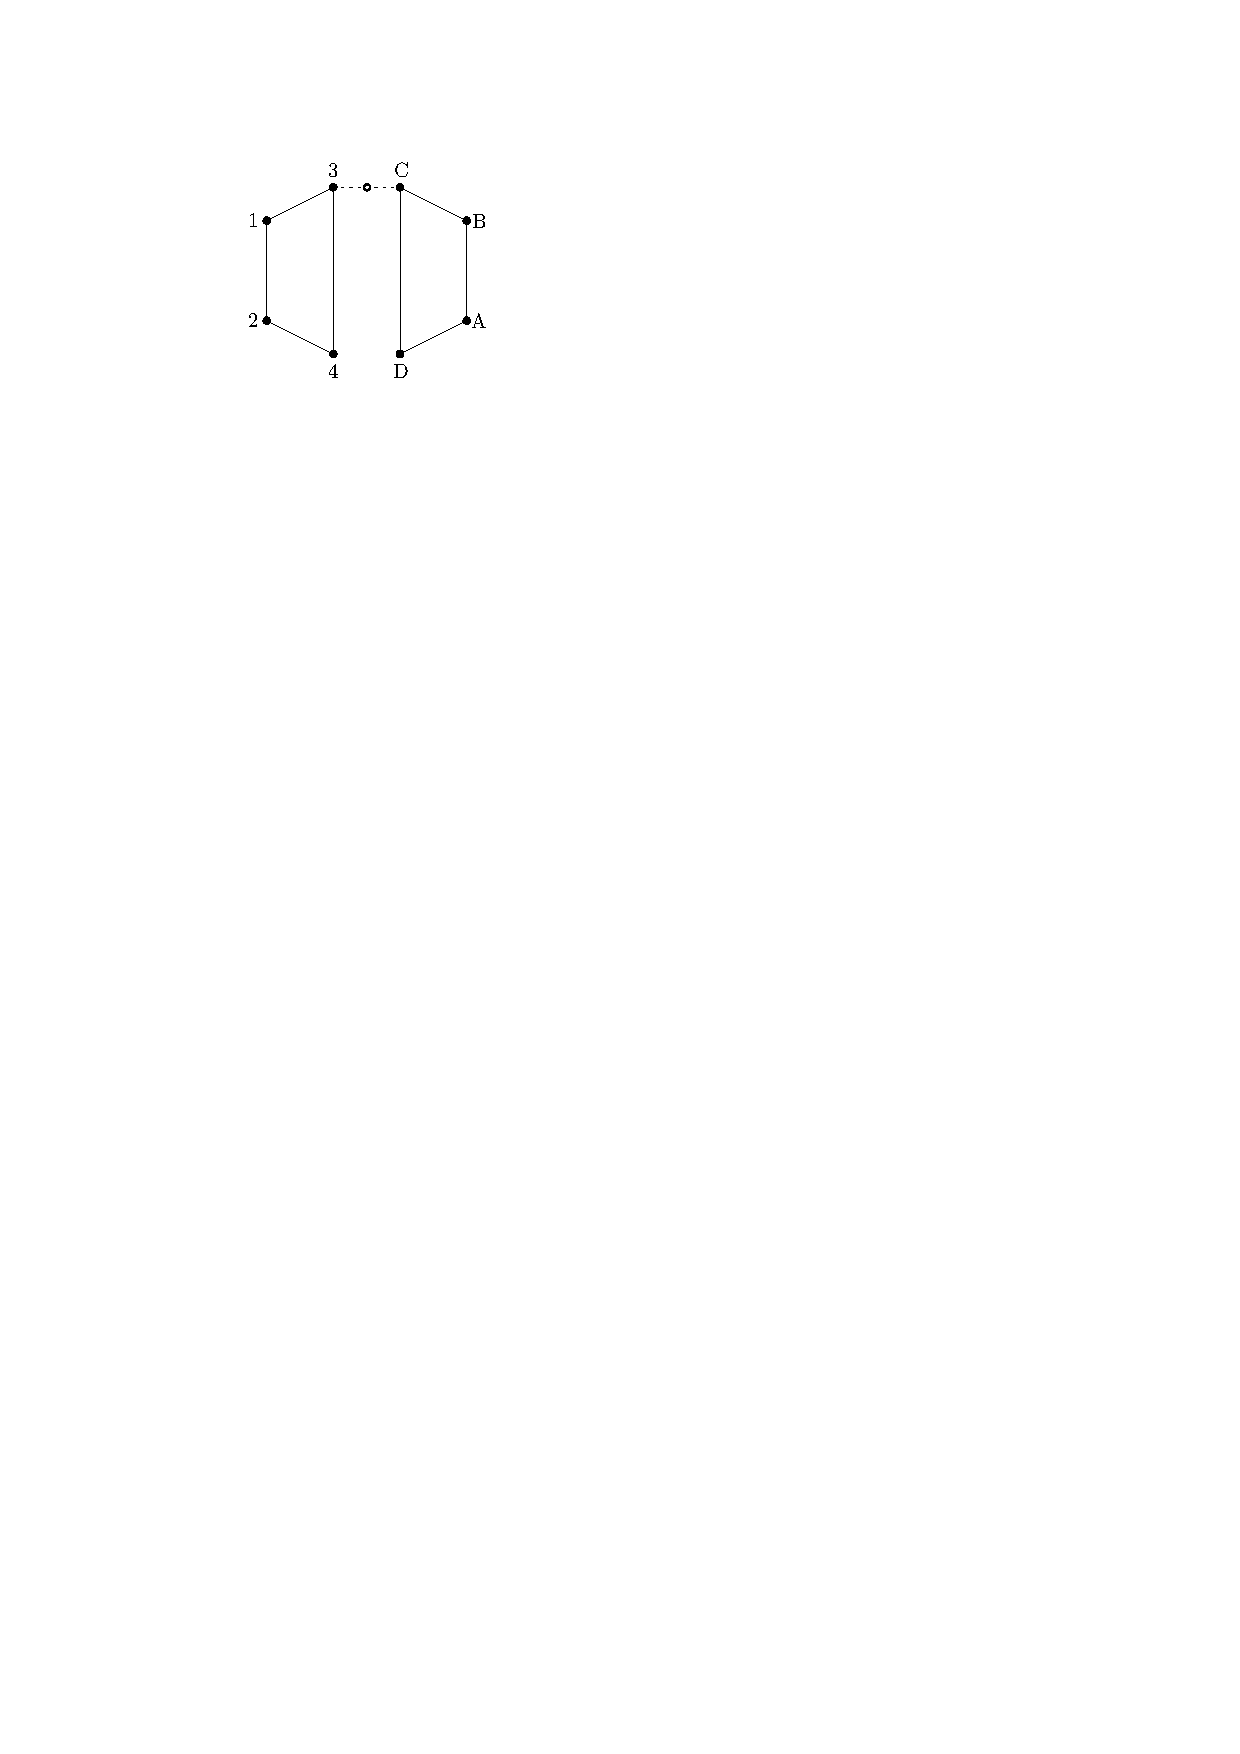
\includegraphics{img/bad-example-1} & 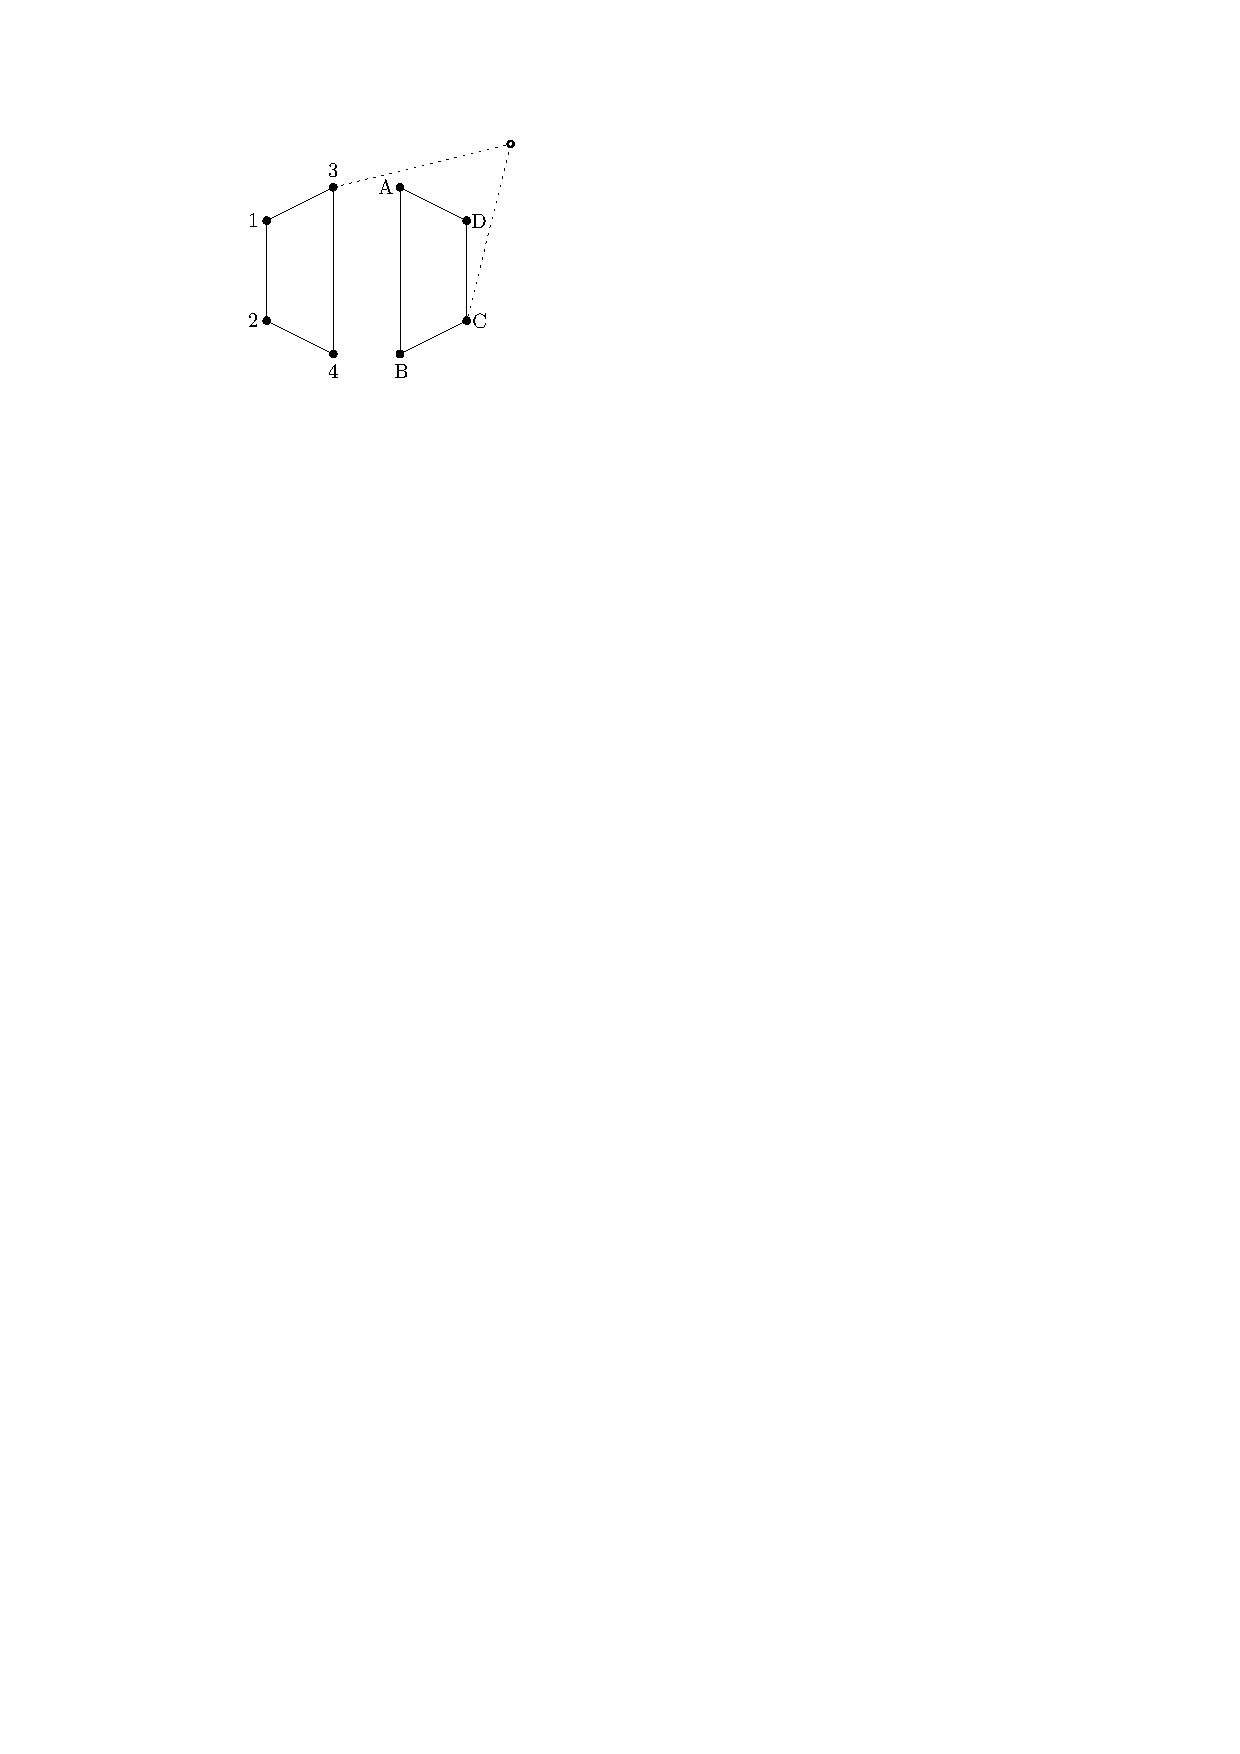
\includegraphics{img/bad-example-2}
    \end{tabular}
  }
  \caption{Two drawings of the same graph, $\mathcal{G}$, where making $\mathcal{G}$ connected requires the addition both of edges and vertices. In this case, $\mathcal G$ is made connected by adding the hollow vertex and two dashed edges.}
  \label{fig:bad-example}
\end{figure}

The motivation for studying this problem comes the problem of morphing
planar graphs, which has many applications \cite{erten.kobourov.ea:intersection,friedrich.eades:graph,gotsman.surazhsky:guaranteed,surazhsky.gotsman:controllable,surazhsky.gotsman:intrinsic} including
computer animation.  Imagine an
animator who wishes to animate a scene in which a character's expression
goes from neutral, to surprised, to happy. The animator can draw these
three faces, but does not want to hand-draw the 30--60 frames required
to animate the change of expression.  The strokes used to draw the
character's features can be converted into paths and these can be merged
into components corresponding to the character's eyes, nose, mouth and
so on.  A correspondence between the same elements in different pictures
is also given.\footnote{In many cases, the correspondence is a byproduct
of the creation process. For example, in the Figure~\ref{fig:faces}, the second
two faces were obtained by copying and then editing the first one.}

\begin{figure}
  \centering{ 
  \begin{tabular}{c@{\hspace{1cm}}c@{\hspace{1cm}}c}
    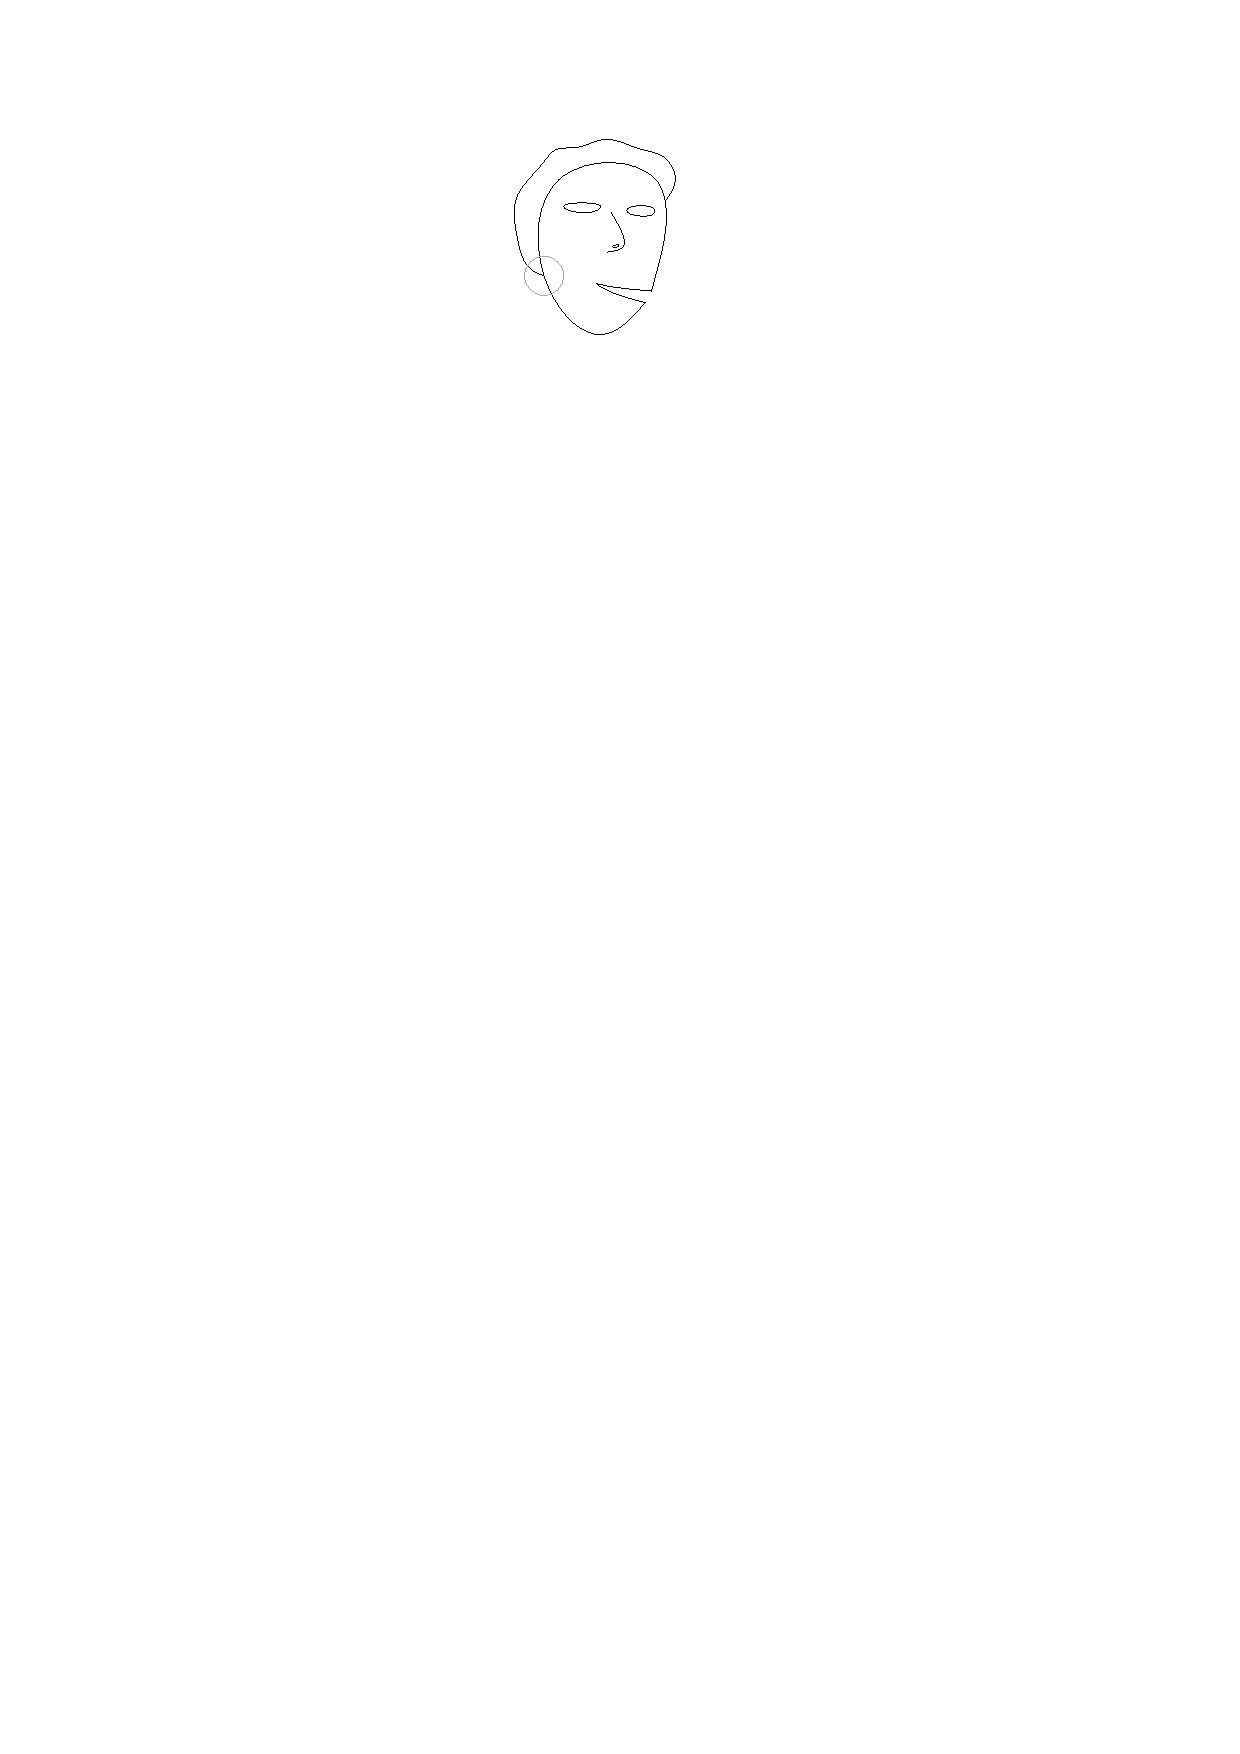
\includegraphics{img/faces-1} &
    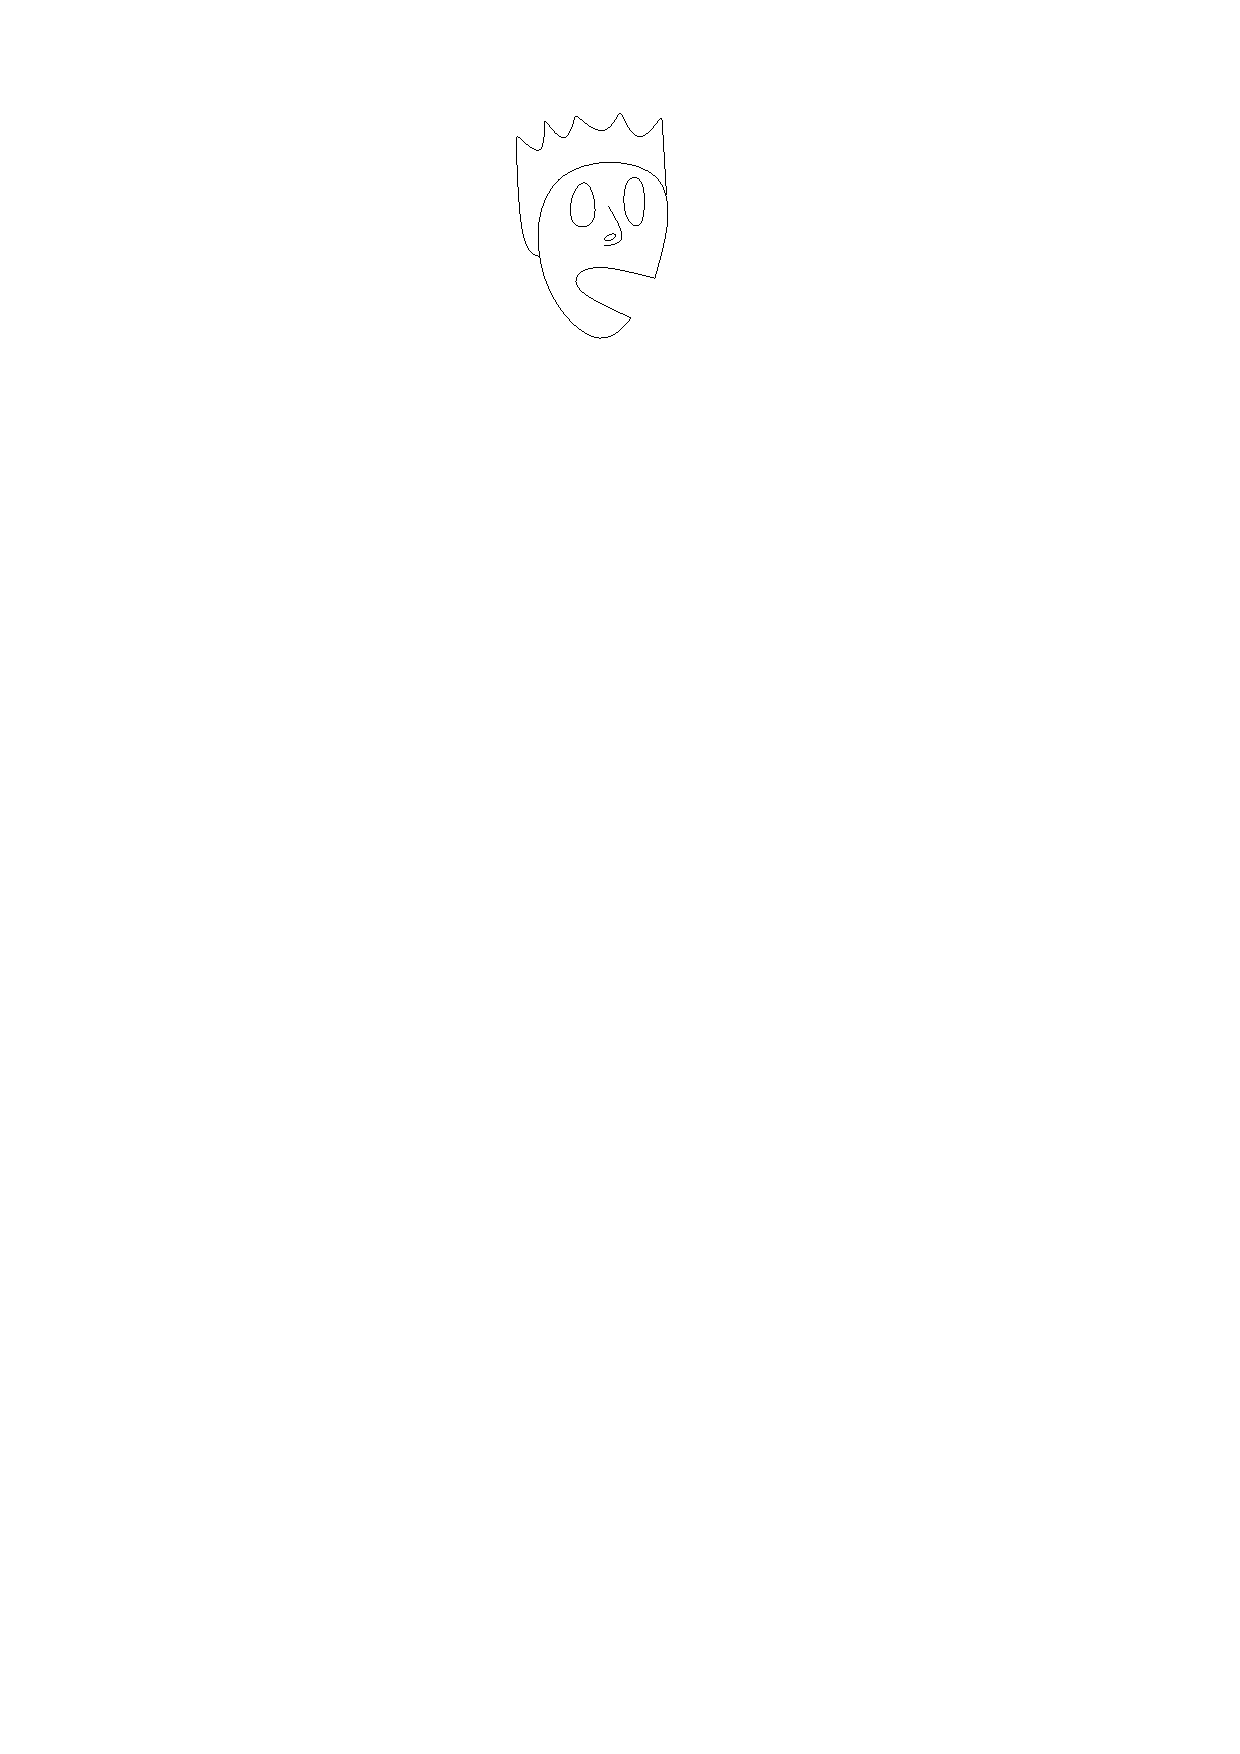
\includegraphics{img/faces-2} &
    
\includegraphics{img/faces-3} \\
    & 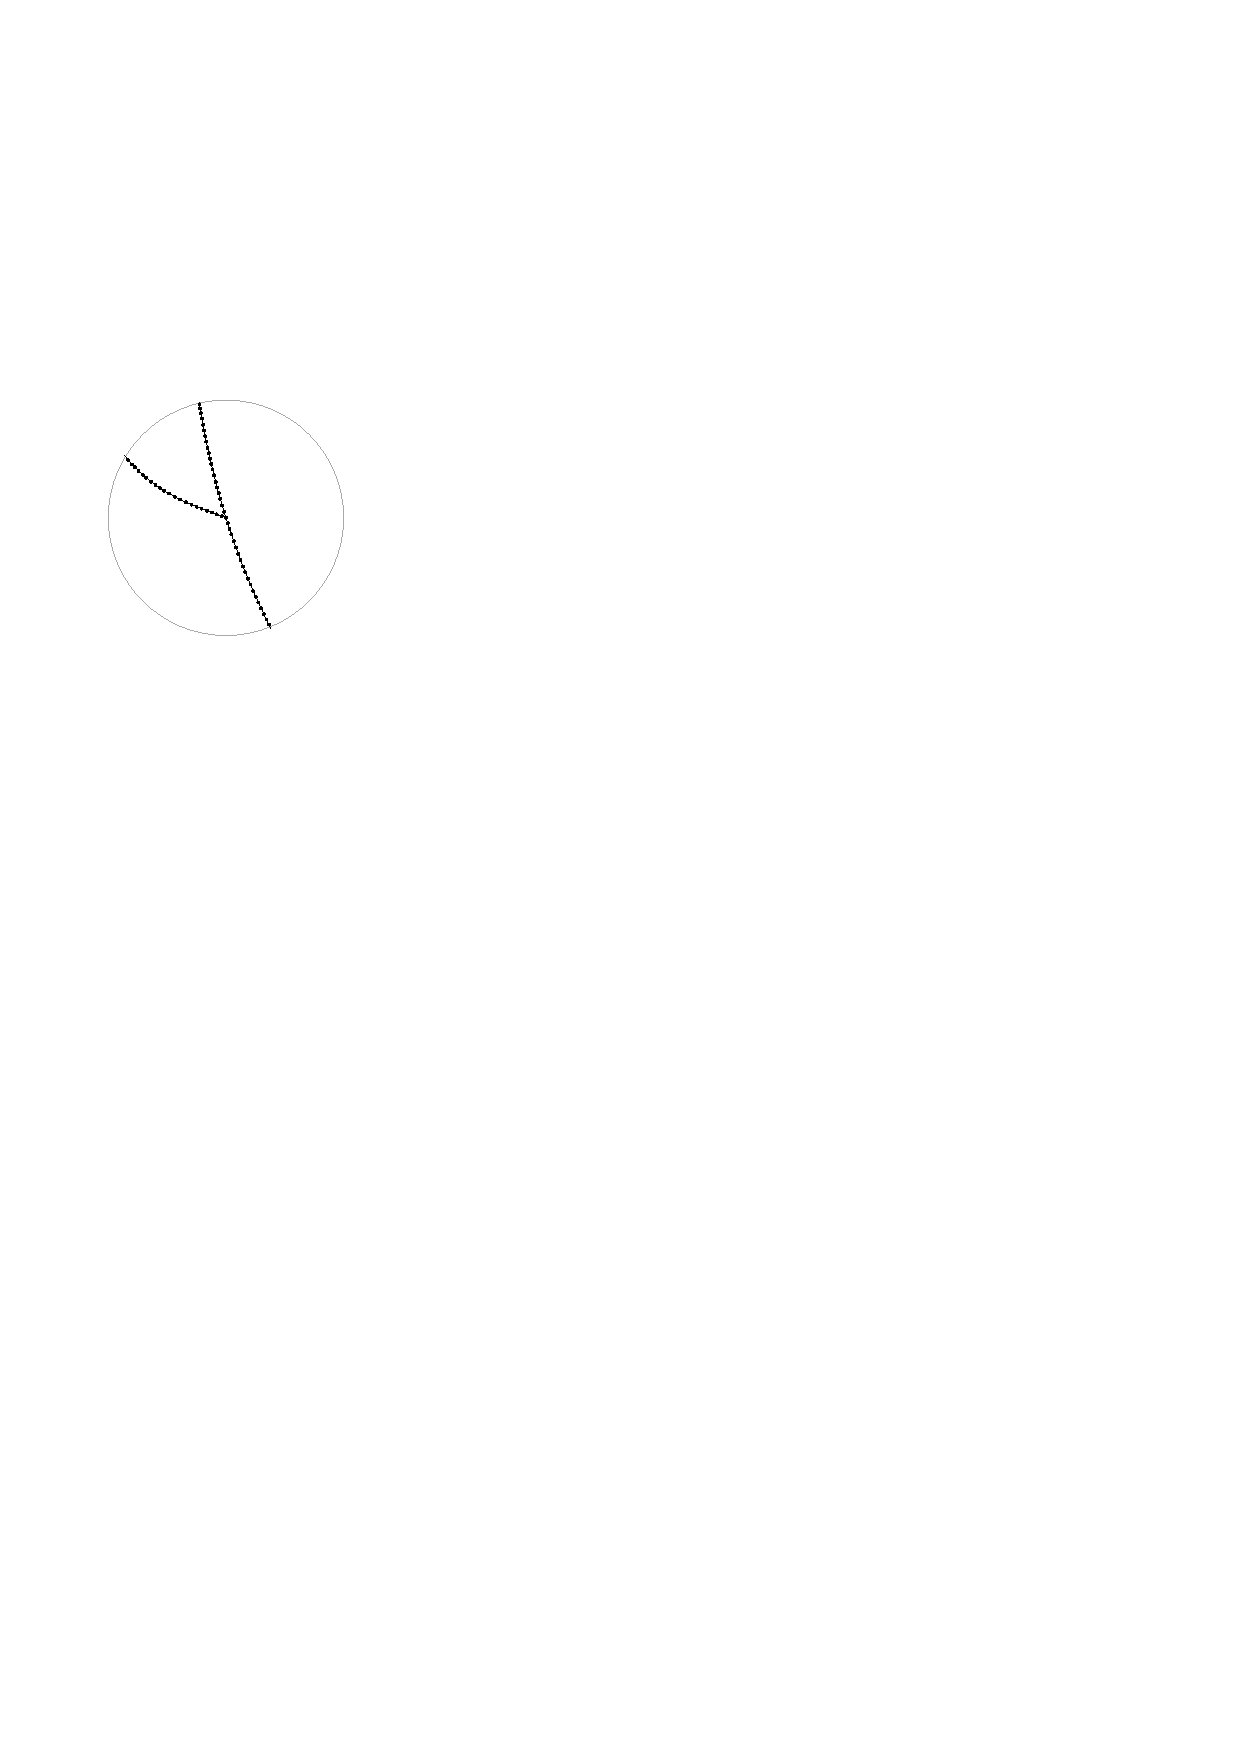
\includegraphics{img/face-zoom} &
  \end{tabular}}
  \caption{Computer-assisted animation frequently involves morphing between
   a sequence of embeddings of the same planar graph.  Zooming in on a section
   of the image reveals that the artist's strokes are approximated by polygonal
   paths}
  \label{fig:faces}
\end{figure}

In this setting, animating the face becomes a problem of \emph{morphing}
(i.e., continuously deforming) one drawing of a planar graph into
another drawing of the same planar graph while maintaining planarity
of the drawing throughout the deformation. This morphing problem
has been studied since 1944, when Cairns \cite{cairns:deformations} showed such a
transformation always exists between any two drawings of the same graph.
Since then, a sequence of results has shown that such transformations
can be done efficiently, so that the motion can be described concisely
\cite{thomassen:deformations, grunbaum.shephard:geometry,alamdari.angelini.ea:morphing, angelini.dalozzo.ea:morphing}.
The most recent such result \cite{angelini.dalozzo.ea:morphing} shows that any
planar drawing of a $n$-vertex connected planar graph can be morphed
into any compatible drawing\footnote{Two drawings of the same graph are
compatible if they have the same ordering of edges around vertices and
the same structure of faces; see Section~\ref{sec:X}.} of the same planar
using a sequence of $O(n)$ \emph{linear morphs}, in which vertices move
along linear trajectories at constant speed.

These morphing algorithms require that the input graph, $\mathcal{G}$,
be connected. In many applications of morphing (for example in
Figure~\ref{fig:faces}) the input graph is not connected. Before these
morphing algorithms can be used, $\mathcal{G}$ must be augmented into a
connected graph, $\mathcal H$, but this augmentation must be compatible
with the drawings of $\mathcal{G}$.  At the same time, the complexity
of the morph produced by a morphing algorithm depends on the number
of vertices of $\mathcal H$.  Therefore, we want to find an augmentation
with the fewest number of vertices.

This raises the question studied in the current paper:  How can we add
vertices and edges to $\mathcal{G}$ to obtain a supergraph $\mathcal
H\supset \mathcal G$ that is connected and such that the vertices and
edges of $\mathcal{H}$ can also be added to the drawings of $\mathcal{G}$
while maintaining the planarity of each drawing?  In this paper,
we obtain a tight bound for the extremal question: In the worst-case
(over all $n$ vertex planar graphs, $\mathcal G$, and over all sets of
$k$ planar drawings of $\mathcal{G}$), how many edges have to be added
to $\mathcal{G}$ to obtain connectivity while preserving planarity of
the drawings?


\subsection{Formal Problem Statement and Main Result}


Let $\mathcal G$ be a planar graph with $n$ vertices and $r$ connected
components.  Given $k$ geometric planar isomorphic embeddings $G_1,
\ldots, G_k$ of $\mathcal G$, a \emph{compatible augmentation},
$\mathcal H$, of $\mathcal G$ is a supergraph of $\mathcal G$ such that
(1) $\mathcal H$ is connected, and (2) there exist geometric planar
isomorphic embeddings, $H_1, \ldots, H_k$, of $\mathcal H$ such that
$H_i\supset G_i$ for every $1\leq i\leq k$.  In this paper, we show
that $G$ always has a compatible embedding of size $O(nr^{1-1/k})$
and that this bound is tight; there exists a graph $\mathcal G$ with $r$
components and having embeddings $G_1,\ldots,G_k$ for which any compatible
augmentation has size $\Omega(nr^{1-1/k})$.

\red{This needs more details.  In particular, we need to properly define planar isomorphic embeddings. Yuck!}

\subsection{Related Work}

To the best of our knowledge, there is very little work on
compatible connectivity-augmentation of planar graphs, though
there is work on isomorphic triangulations of polygons.  Refer to
Figure~\ref{fig:compatible-triangs}.  In this setting, the graph $\mathcal{G}$
is a cycle and one has two non-crossing drawings, $P$ and $Q$, of
$\mathcal G$ The goal is to augment $\mathcal G$ (and the two drawings
$P$ and $Q$) so that $G$ becomes a near-triangulation, and $P$ and $Q$
become (geometric) triangulations of the polygons whose boundaries are
$P$ and $Q$.  Aronov \etal\ \cite{aronov.seidel.ea:compatible} showed that this
can always be accomplished with the addition of $O(n^2)$ vertices and
that $O(n^2)$ vertices are sometimes necessary.  Kranakis and Urrutia
\cite{kranakis.urrutia:isomorphic} showed that this result can be made sensitive
to the number of reflex vertices of $P$ and $Q$, so that the number
of triangles required is $O(n+pq)$ where $p$ and $q$ are the number of
reflex vertices of $p$ and $q$, respectively.

\begin{figure}
  \centering{
    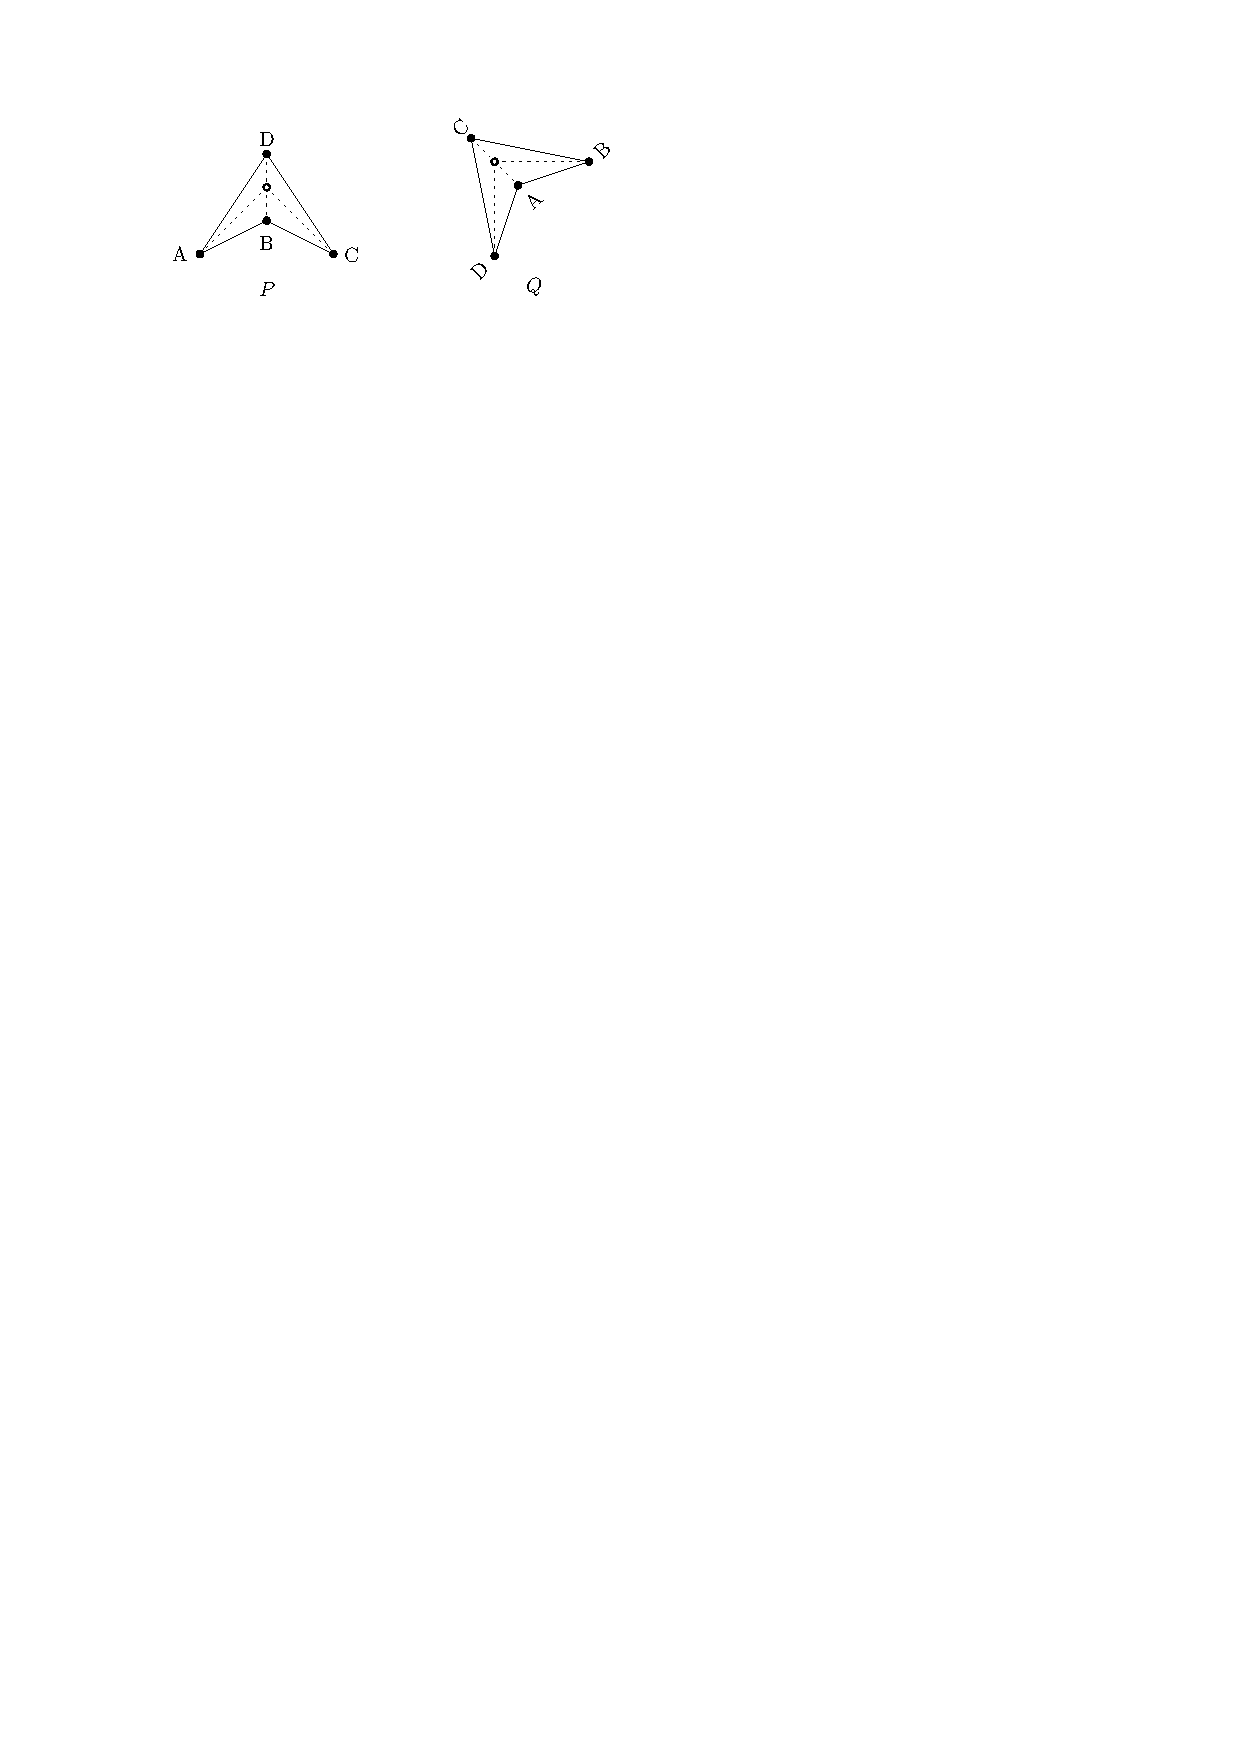
\includegraphics{img/compatible-triangs}
  }
  \caption{Compatible triangulations of two polygons $P$ and $Q$.}
  \label{fig:compatible-triangs}
\end{figure}

Babikov \etal\ \cite{babikov.souvaine.ea:constructing} showed that the result of Aronov \etal\ can be extended to polygons with holes. This work is the most closely related to ours because it encounters our problem as a subproblem. In their setting, the graph $\mathcal G$ is a collection of cycles and the embeddings $P$ and $Q$ are such that one cycle of $\mathcal G$ contains all the others in its interior.  In the first stage of their algorithm, they build a connected supergraph $\mathcal{H}'$ of $\mathcal{G}$, but their supergraph has size $\Theta(n^2)$ in the worst-case.  A byproduct of our main theorem is that this step of their algorithm could be done with a graph $\mathcal{H}'$ having only $O(n^{3/2})$ edges (but completing this graph to a triangulation may still require $\Omega(n^2)$ edges).

\red{We should mention, maybe later on, that they have to solve similar routing problems as us; they have two paths along the boundaries of $P$ and $Q$ that visit the components in the wrong order.}

\section{Upper bounds for trivial components}\label{section:Trivial components}
To provide some intuition, we start by showing the result for the case when $\mathcal G$ is a graph containing $n$ vertices and no edges, i.e., $\mathcal G$ contains $n$ (trivial) connected components. Before constructing the compatible augmentations, we provide a subroutine that constructs a ``short'' plane spanning path of a point set. Later, we use this subroutine on each of the geometric drawings of $\mathcal G$ to obtain isomorphic compatible augmentations of bounded length.


%%%%%%%%%
\subsection{Spanning paths of point sets}
Let $S$ be a set of $n$ points in the plane such that no two points of $S$ have the same $x$-coordinate. 
Given a point $v\in S$, let $rank(v)$ denote the number of points of $S$ that lie to the left of $v$.

Given an arbitrary order $(v_1, v_2, \ldots, v_n)$ of the points of $S$, we want to construct a path $R$ that connects them in the given order such that:  $$|R|  = O\left(\sum_{i=1}^{n-1} |rank(v_i) - rank(v_{i+1})| \right).$$

Consider a horizontal line such that each point of $S$ lies above it and let $\pi$ be the closed halfspace supported by this line that contains $S$. After each round of the algorithm, we maintain the invariant that the boundary of $\pi$ does not intersect $R$.

Throughout, we maintain the \emph{escape invariant} which states that for each point $v_j\in S \setminus R$, there is a cone $\Delta_j$ with apex $u_j$ such that (1) $u_j$ lies above $v_j$ (or on $v_j$) and has the same $x$-coordinate as $v_j$, (2) $\Delta_j$ contains $v_j$ and no other point of $S$, (3) $\Delta_j$ contains the ray shooting from $v_j$ in the direction of the negative $y$-axis, (4) $\Delta_j$ does not intersect $R$, (5) $\Delta_i$ and $\Delta_j$ are disjoint inside $\pi$.
Before starting the construction, we establish the escape invariant. To do this, for each $0\leq j\leq n$ let $u_j$ be an arbitrary translation of $v_j$ in the direction of the positive $y$-axis and let $\Delta_j$ be a cone with apex on $u_j$ sufficiently narrow such that these cones doe not intersect inside $\pi$; see Figure~\ref{fig:Escape Invariant}.

\begin{figure}[tb]
\centering 
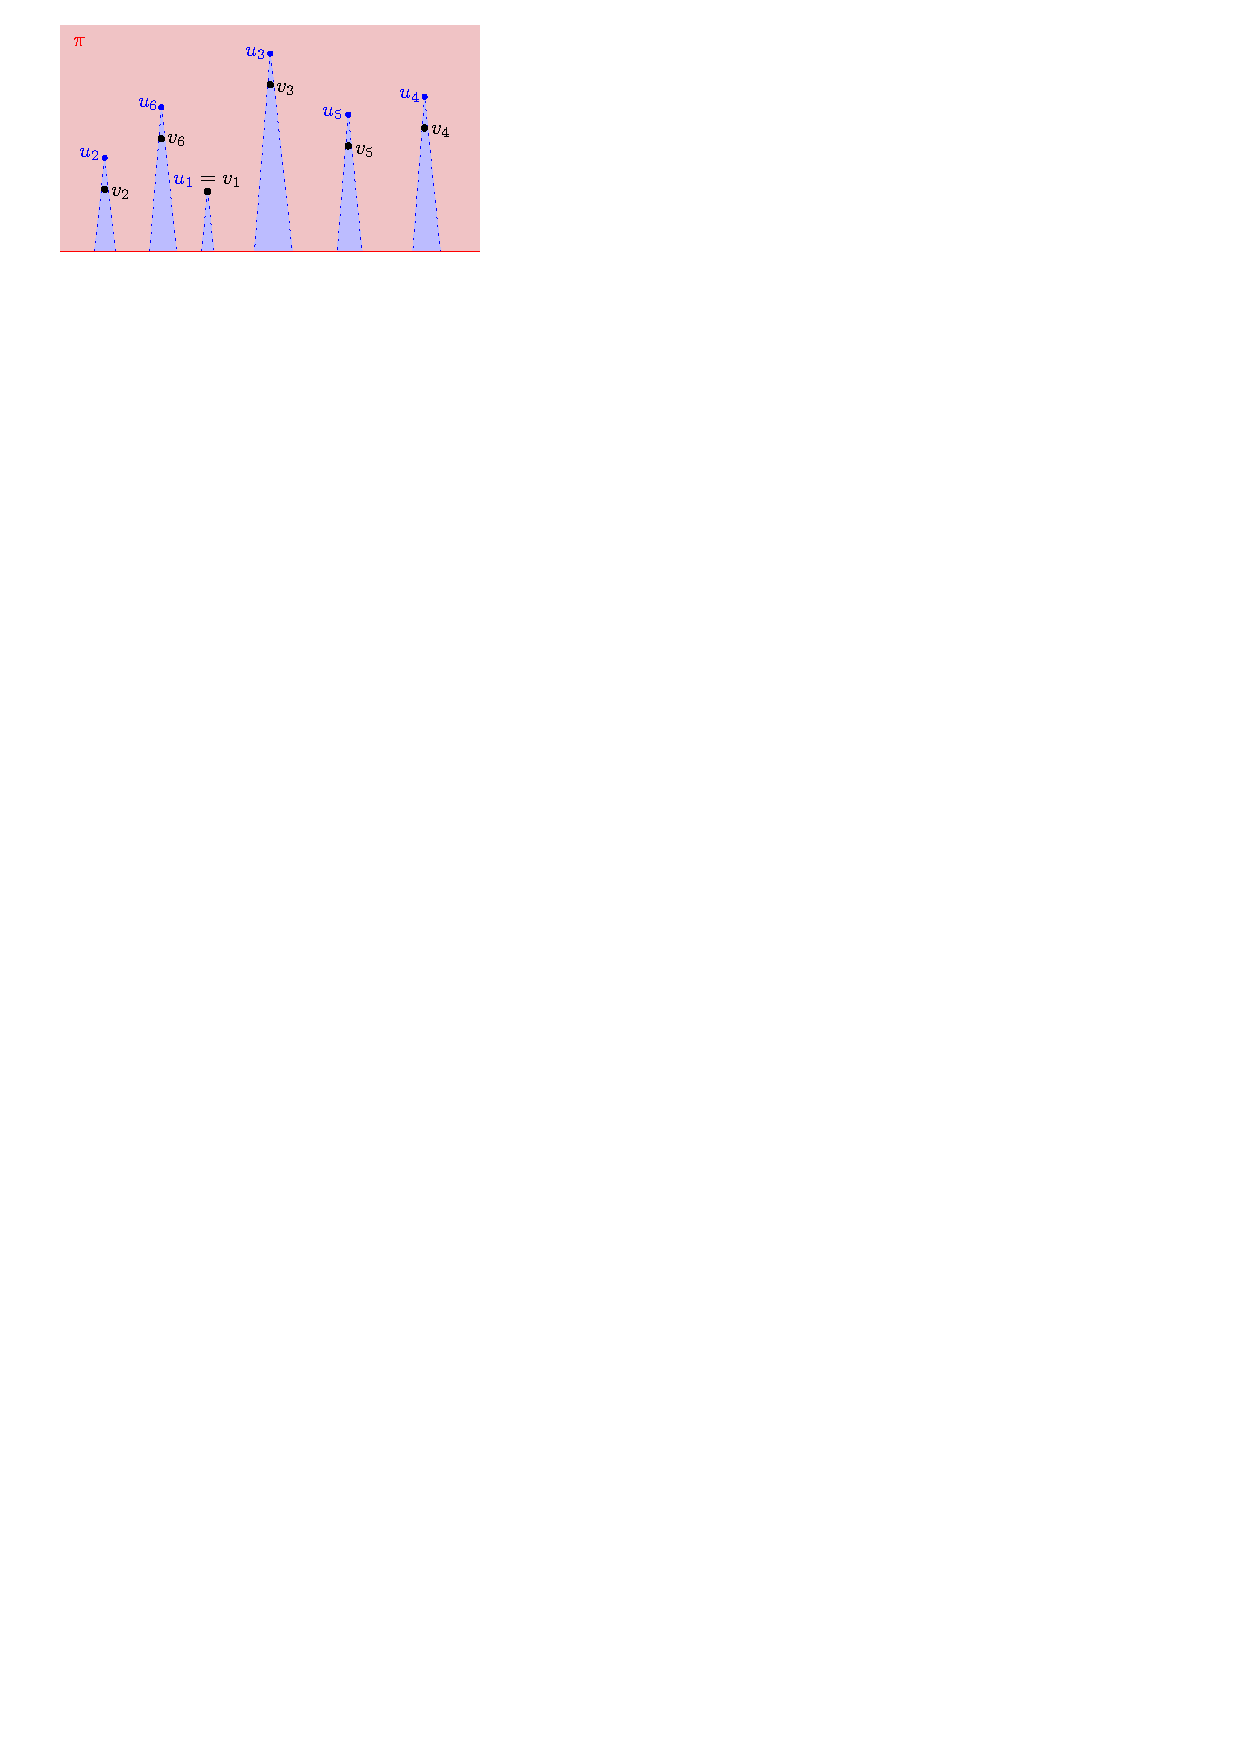
\includegraphics{img/EscapeInvariant.pdf}
%[width=1\textwidth]
\caption{\small }
\label{fig:Escape Invariant}
\end{figure}

To construct $R$, we add the points of $S$, one by one, according to the given order while maintaining the escape invariant.
Assume that $R$ is a path connecting $v_1$ with $v_j$ (initially, $j=1$ and $R$ consists of the single vertex $v_1$).
We extend $R$ by appending a path that connects $v_j$ with $v_{j+1}$. 
As a first step, we translate down the cones $\Delta_j$ and $\Delta_{j+1}$ until their apexes $u_j$ and $u_{j+1}$ coincide with $v_j$ and $v_{j+1}$, respectively. Moreover, we narrow the cone $\Delta_j$ while keeping the ray shooting downwards from $v_j$ contained in $\Delta_j$.

Let $\pi_j$ be the closure of the set obtained from $\pi$ by removing every cone $\Delta_h$, where $1\leq h\leq n$ and $v_h$ is not an internal vertex of $R$; see Figure~\ref{fig:Dented Halfspace}. That is, $\pi_j$ is a halfspace with dents made by the remotion of $n-j+1$ cones.
Therefore, the length of the boundary of $\pi_j$ is $O(n-j)$. 
Moreover, the distance between two apexes $u_i$ and $u_h$ along the boundary of $\pi_j$ is proportional to the number of apexes with $x$-coordinate between that of $u_i$ and $u_h$. That is, the length of the path that joins $u_i$ with $u_h$ along $\pi_j$ is $O(|rank(v_i) - rank(v_h)|)$. 

\begin{figure}[tb]
\centering
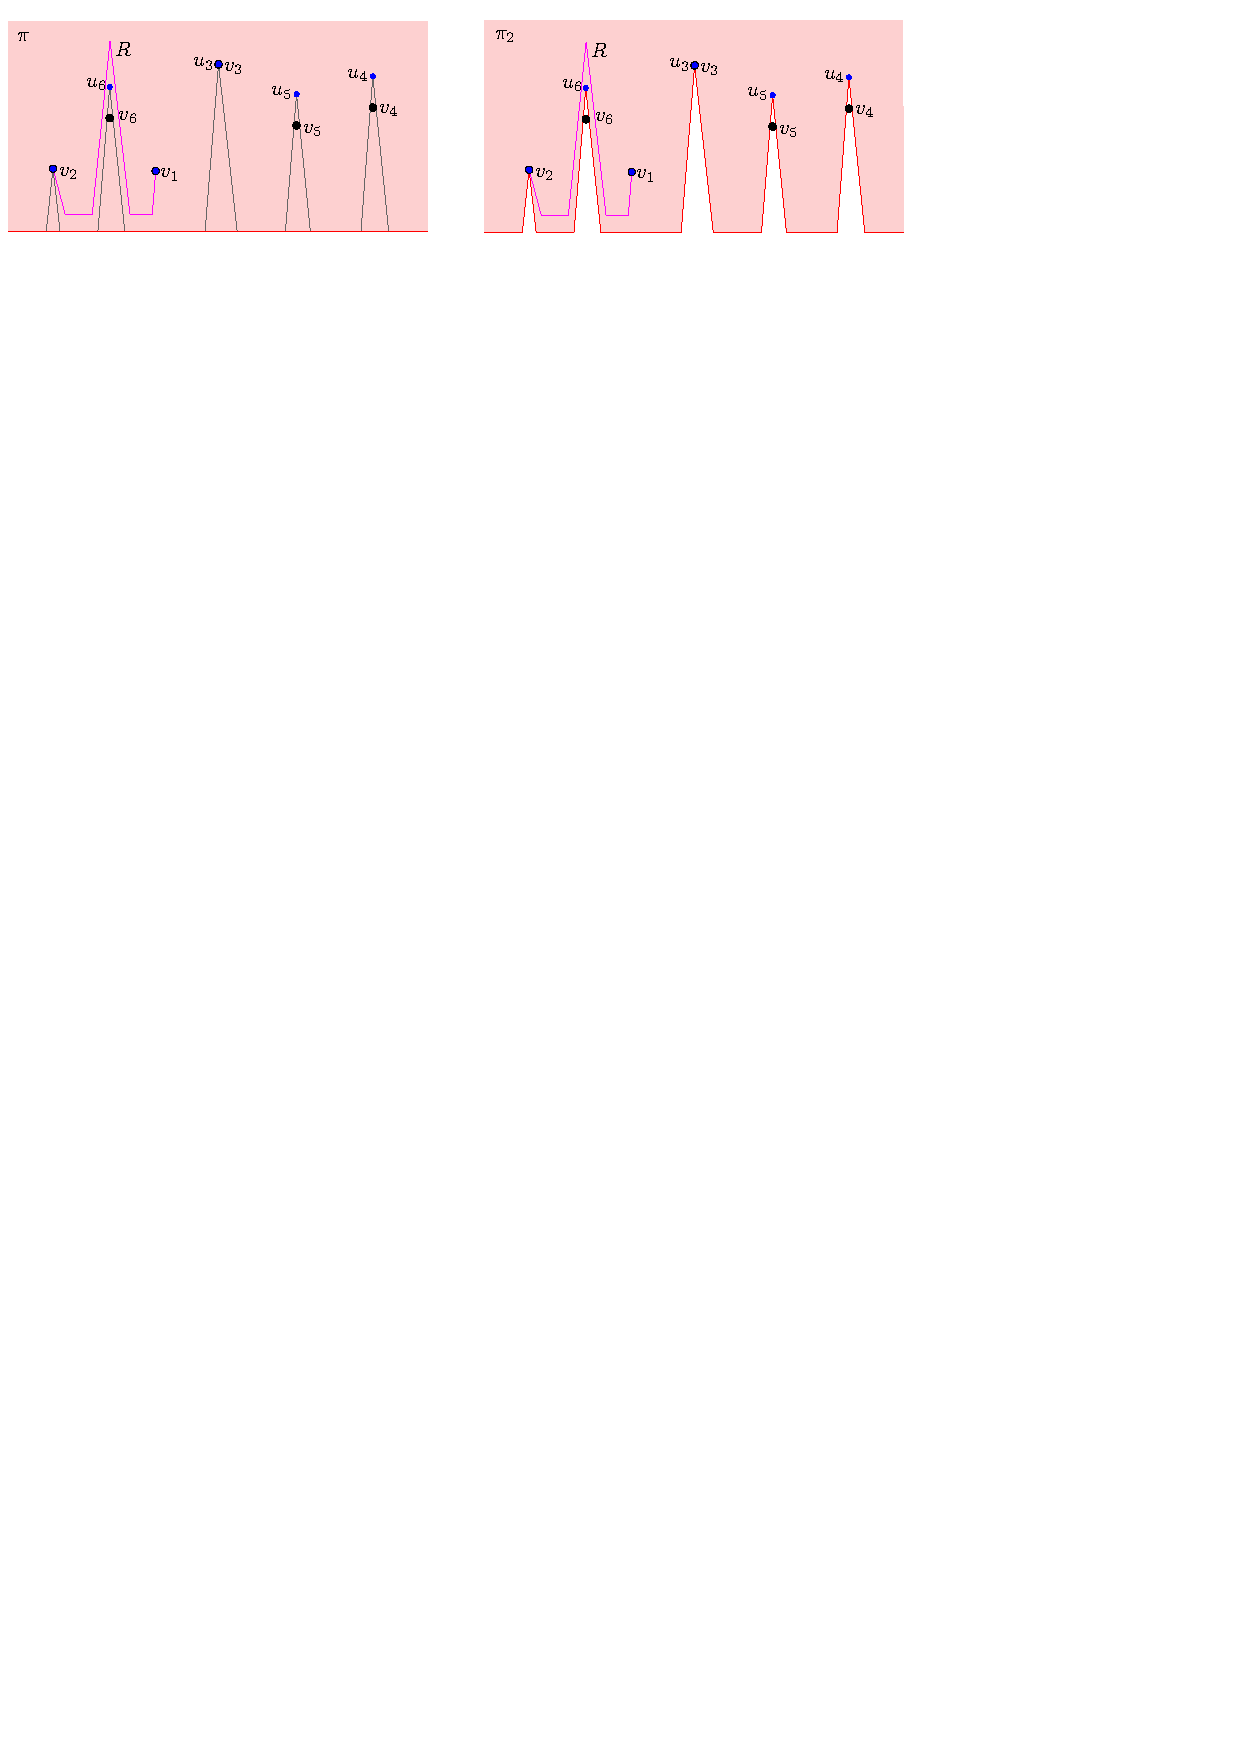
\includegraphics[width=1\textwidth]{img/DentedHalfspace.pdf}
%[width=1\textwidth]
\caption{\small }
\label{fig:Dented Halfspace}
\end{figure}


Because the boundary of $\pi$ does not intersect $R$ and by property (4) of the escape invariant, the boundary of $\pi_j$ intersects the portion of $R$ constructed so far only at $v_j$. Moreover, by property (2) of the escape invariant, each point of $S\setminus V(R)$ lies outside of~$\pi_j$ except for $v_{j+1}$ that lies on its boundary.
Because both $v_j$ and $v_{j+1}$ lie on the boundary of $\pi_j$ and since this boundary does not intersect the interior of $R$, we can connect $v_j$ with $v_{j+1}$ with a path contained in the boundary of $\pi_j$. 
Recall that this path has length $O(|rank(v_j) - rank(v_{j+1})|)$. In this way, we extend $R$ to a planar path that connects $v_1$ with $v_{j+1}$.

After connecting $v_j$ with $v_{j+1}$, for each $v_h\notin R$, either $\Delta_h$ is disjoint from $R$, or it shares some portion of its boundary with $R$. However, the interior of $\Delta_h$ does not intersect $R$.
To preserve the escape invariant, for each $1\leq h\leq n$ such that $v_h\notin R$, translate the cone $\Delta_h$ downwards a distance $\varepsilon>0$. Because the translated cone is contained in the previous one and since its apex $u_h$ lies above $v_h$ by property (1) of the escape invariant, by choosing $\varepsilon$ sufficiently small, we guarantee that the escape invariant is maintained. Similarly, we move $\ell$ a distance $\varepsilon$ in the direction of the negative $y$-axis. Using this algorithm repeatedly until all points of $S$ are connected, we obtain the following result.

\begin{lemma}\label{lemma:Compatible augmentation for trivial components}
Given an arbitrary order $(v_1, \ldots, v_n)$ of the vertices of $S$, the previous algorithm computes a plane path $R$ that connects every point of $S$ in the given order such that 
$|R| = O\left(\sum_{i=1}^{n-1} |rank(v_i) - rank(v_{i+1})| \right)$. 
\end{lemma}
\begin{proof}
Recall that in each iteration, the algorithms computes a path connecting $v_j$ with $v_{j+1}$ that does not cross the portion of the path already constructed. Because this invariant is maintained throughout, the resulting path is planar.

Since the path that connects $v_j$ with $v_{j+1}$ follows the boundary of $\pi_j$ and since this boundary has length $O(|rank(v_j) - rank(v_{j+1})|)$ between $v_j$ and $v_{j+1}$, the path that connects $v_j$ with $v_{j+1}$ has length $O(|rank(v_j) - rank(v_{j+1})|)$. Consequently,  the total length of $R$ is given by $O\left(\sum_{i=1}^{n-1} |rank(v_i) - rank(v_{i+1}) |\right)$.
\end{proof}



\subsection{Compatible drawings of point sets}
Recall that in this section, $\mathcal G$ is a graph with $n$ trivial components.
Let $G_1, \ldots, G_k$ be $k$ isomorphic drawings of $\mathcal G$, i.e., $G_i$ is a set of $n$ points in the plane.
Assume without loss of generality that no two points of $G_i$ share the same $x$-coordinate. Otherwise, rotate the coordinate system slightly.
Given a vertex $v$ of $\mathcal G$, let $rank_{G_i}(v)$ denote the number of points of $G_i$ to the left of $v$.

For each $v$ of $\mathcal G$, let $x_v = (rank_{G_1}(v), rank_{G_2}(v), \ldots, rank_{G_k}(v))$ be a point in the integer grid of side-length $n$ contained in $\mathbb{R}^k$.
Let $X = \{x_v : v\in V(\mathcal G)\}$ and let $P$ be the shortest hamiltonian path of $X$, i.e., the shortest path that visits every point of $X$.
It is known that the length of $P$ is $O(n^{2-1/k})$~\cite{}.

Note that the order of the points of $P$ induces an order on the vertices of $\mathcal G$ and hence, an order on the points of each $G_i$. 


\begin{theorem}
For each $1\leq i\leq n$, we can construct a path $R_i$ of length $O(n^{2-1/k})$ that connects every point of $G_i$ such that $G_i\cup R_i$ is plane. Moreover, for each $1\leq i < j \leq n$, $G_i\cup R_i$ is isomorphic to $G_j\cup R_j$.
\end{theorem}
\begin{proof}
For each $G_i$, we use Lemma~\ref{lemma:Compatible augmentation for trivial components} to construct a plane path $R_i$ that connects the points of $G_i$ in the order induced by $P$.
Assume that $(v_1, \ldots, v_n)$ is the order of the points of $G_i$ induced by $P$.
Therefore, $|R_i| = O\left(\sum_{j=1}^{n-1} |rank_{G_i}(v_j) - rank_{G_i}(v_{j+1}) |\right)$.
Note that the if $d_j$ denotes the distance between $x_{v_j}$ and $x_{v_{j+1}}$ along $P$, then
$|rank_{G_i}(v_j) - rank_{G_i}(v_{j+1})|\leq  d_j$. 
Therefore, the path contained in $R_i$ that connects $v_j$ with $v_{j+1}$ has length $O(d_j)$. 
Because $\sum_{j=1}^n d_j = |P| = O(n^{2-1/k})$, the total length $R_i$ is $O(n^{2-1/k})$.

Since the vertices of each $G_i$ are connected in the same order, $G_i\cup R_i$ is isomorphic to $G_j\cup R_j$ for each $1\leq i<j\leq n$.
\end{proof}


\section{The general problem}
In this section, we extend the result presented in Section~\ref{section:Trivial components} to graphs with non-trivial components.
As in Section~\ref{section:Trivial components}, we provide a subroutine that constructs a path connecting all components of a plane graph in any given order.

\subsection{Preliminaries}\label{section:Preliminaries}
Let $C$ be a connected geometric plane graph. Let $v_0, v_1, \ldots, v_k, v_0$ be the sequence of vertices of $C$ visited by a counterclockwise Eulerian tour along the boundary of $C$. Note that $v_i$ may be equal to $v_j$ for some $i\neq j$. 
A vertex of $v_i$ in this sequence is called a \emph{corner} of $C$.
In this paper, we consider the boundary of $C$, denoted by $\partial C$, to be the boundary of the weakly-simple polygon $(v_0, \ldots, v_k, v_0)$ whose vertex set is the set of corners of $C$.

Let $\varepsilon >0$. For each cornet $v_i$ of $\partial C$,
let $\ell_i$ be the line passing through $v_i$ that bisects the angle between the edges $v_{i-1}v_i$ and $v_i v_{i+1}$.
Let $z_i$ be the point at distance $\varepsilon$ from $v_i$ along $\ell_i$ such that $v_{i-1} v_i z_i$ either makes a right turn or defines three collinear points such that $v_i\in [v_{i-1}, z_i]$. We call $z_i$ the \emph{$\varepsilon$-copy} of $v_i$.
Let $\partial_\varepsilon C$ be the polygon defined by the sequence $(z_0, z_1, \ldots, z_k, z_0)$, i.e., $\partial_\varepsilon C$ is isomorphic to $\partial C$. We call $\partial_\varepsilon C$ the \emph{$\varepsilon$-fattening} of $C$.
An $\varepsilon$-fattening $\partial_\varepsilon C$ is \emph{simple} if $\partial_\varepsilon C$  is a simple polygon that contains~$C$.
Note that $\partial_\varepsilon C$ is simple, provided that $\varepsilon$ is sufficiently small. In this paper, we consider only simple $\varepsilon$-fattenings; see Figure~\ref{fig:Blowing}. Note that the (graph) distance between two corners of $\partial C$ along the boundary of $C$ is the same as the distance between their $\varepsilon$-copies along~$\partial_\varepsilon C$.

\begin{figure}[tb]
\centering
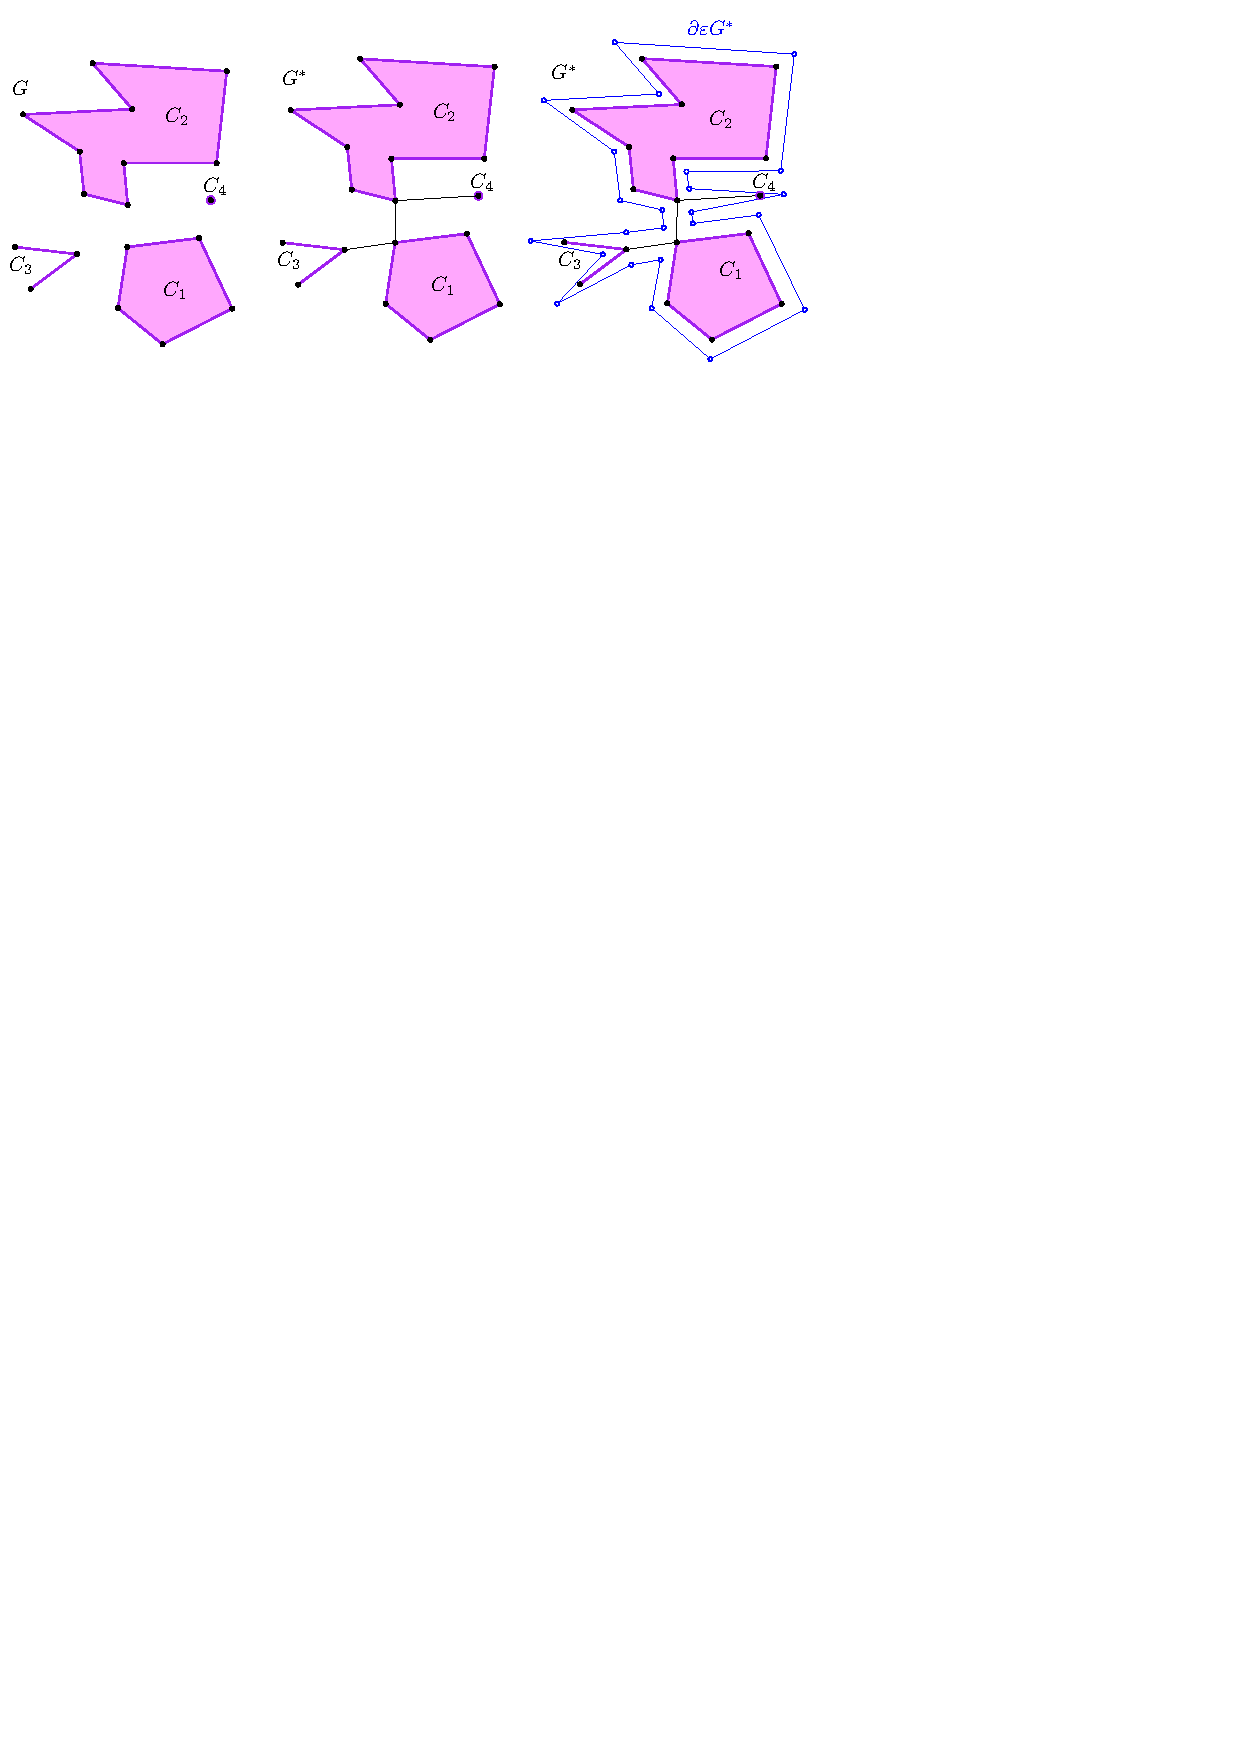
\includegraphics{img/Blowing.pdf}
%[width=1\textwidth]
\caption{\small }
\label{fig:Blowing}
\end{figure}

%%%%%%%%%%%%%%%
\subsection{Connected augmentations}\label{section: connected augmentations}
Let $G$ be a geometric plane graph with $r$ connected components such that each component is adjacent to the outer face.
Consider the visibility graph of $G$ where two vertices are visible if the open segment joining them does not intersect $G$.
Let $T_G$ be a smallest set of edges of the visibility graph of $G$ that need to be added to $G$ to make it connected.
Because there are always two components visible from each other, we can connect them and repeat recursively with one less component. Therefore, $r-1$ edges are always sufficient to connect all the components of $G$. Moreover, because $G$ has $r$ connected components, $T_G$ consists of exactly $r-1$ edges.
Let $G^* = G\cup T_G$. Note that $\partial G^*$ consists of at most  $n+r-1$ edges.
We say that $G^*$ is a \emph{connected augmentation} of $G$; see Figure~\ref{fig:Blowing}.

Let $C_1, \ldots, C_r$ be the components of $G$. 
Recall that we consider $\partial C_i$ to be the boundary of a weakly-simple polygon. Therefore, even though a vertex of $C_i$ can appear multiple times along $\partial C_i$, we consider them as different corners of $\partial C_i$. 
For each $1\leq i\leq r$, let $a_i\in C_i$ be an arbitrary corner of $\partial C_i$ (note that $a_i$ is adjacent to the outer face).
We call $a_i$ the \emph{attachment corner} of $C_i$.

Let $\varphi$ be the path obtained by splitting $\partial G^*$ at the corner $a_1$. 
That is, $\varphi$ is a path with both endpoints equal to $a_1$. 
Moreover, we assume that $\varphi$ is oriented in counterclockwise order along $\partial G^*$.
Note that $\varphi$ visits every corner of $\partial G^*$ exactly once except for $a_1$.

Given two corners $u$ and $v$ in $\partial G^*$, let $\varphi(u,v)$ denote the shortest path contained in $\varphi$ that connects $u$ with $v$. Let $A(u,v)$ be the set of attachment corners of $G$ visited by $\varphi(u,v)$. 
Let $\sigma_G(u,v) = |\varphi(u,v)| + \sum_{a_i\in A(u,v)} |C_i|$ be the \emph{cost} of going from $u$ to $v$.


\begin{lemma}\label{lemma:Contained in integer grid}
If $a$ is an attachment corner of $G$, then $\sigma_G(a_1, a) \leq 5n$. Moreover, if $b$ is another attachment corner of $G$, then $\sigma_G(a, b) =  |\sigma_G(a_1, a)- \sigma_G(a_1, b)|$. 
\end{lemma}
\begin{proof}
Because $|\partial G^*| \leq n + r-1$ and from the fact that $ |\varphi(a_1,a)| \leq |\varphi| = |\partial G^*|$, we know that $|\varphi(a_1,a)|\leq n + r-1$.
Therefore, since $\sum_{i = 1}^r |\partial C_i|\leq |E(G) | \leq 3n$, we conclude that $\sigma_G(a_1, a)  = |\varphi(a_1,a)| + \sum_{a_i\in A(a_1,a)} |C_i| \leq 4n + r-1\leq 5n$.

Because each attachment corner of $G$ visited by $\varphi(a_1, a)$ is also visited by $\varphi(a_1, b)$ and from the fact that $ |\varphi(a_1,b)| - |\varphi(a_1, a)| = |\varphi(a, b)|$, we get that 
$\sigma_G(a_1, b)- \sigma_G(a_1, a) = |\sigma_G(a_1, a) - \sigma_G(a_1, b)| = |\varphi(a, b)|  + \sum_{a_i\in A(a, b)} |C_i| = \sigma_G(a, b)$.
\end{proof}

\subsection{Spanning paths for connected augmentations}\label{section:Spanning paths for connected augmentations}
Let $a_1, \ldots, a_r$ be an arbitrary order of the attachment corners of $G$ (we can get the incremental indexing by relabeling the components). 
Given a path $R = (\rho_1, \rho_2, \ldots, \rho_t)$ that passes through all attachment corners of $G$, we say that $C_i$ lies to the right of $R$ if (1) $a_i$ is the only vertex of $C_i$ that belongs to $V(R)$, and (2) if $a_i = \rho_j$ for some $1\leq j\leq t$, then $\rho_{j-1}$ and $\rho_{j+1}$ appear as consecutive vertices when sorting the neighbors of $a_i$ in clockwise order around $a_i$.

We want to construct a path $R$ (possibly containing Steiner vertices) that connects the attachment corners of $G$ in the given order, i.e., if $i < j$, then $a_i$ is visited before $a_j$ by $R$.
We want to construct $R$ in such a way that each component $C_i$ of $G$ lies to the right of~$R$.
Moreover, we want that $|R| = O(\sum_{j=1}^{n-1} \sigma_G(a_j, a_{j+1}))$.
We construct such a path incrementally, starting with the trivial path that contains only $a_1$.

Recall that  for any given $\varepsilon >0$, $\partial_\varepsilon G^*$ denotes the $\varepsilon$-fattening of $G^*$ (see Section~\ref{section:Preliminaries}). 
Let $\mu>0$ be a small constant to be specified later.
Initially, let $\varepsilon = 2\mu$ and let $\delta = \mu/2$. Let $\lambda < \mu/2^{r+1}$ be a constant sufficiently small so that $\partial_\lambda C_i \cap \partial_\lambda C_j = \emptyset$ for each $1\leq i< j\leq r$.
Throughout, $\lambda$ remains constant while $\varepsilon$ and $\delta$ are redefined on each round. However, as an invariant we maintain $\lambda < \delta < \varepsilon$.

For each $1\leq i\leq r$, let $w_i$ be $\varepsilon$-copy of  $a_i$.
Split $\partial_\varepsilon G^*$ at $w_1$, i.e., $\partial_\varepsilon G^*$ is a path with both endpoints equal to $w_1$.
By choosing $\varepsilon$ sufficiently small, we guarantee that $\partial_\varepsilon G^*$ is simple, i.e., $\partial_\varepsilon G^*$ has the same combinatorial structure than $\varphi$.

We say that two points in the plane are \emph{$R$-visible} if the open segment joining them does not intersect $R$.
Let $\tau >0$. For each $1\leq i\leq r$ such that $a_i$ is not an interior point of $R$, consider the set of points $N_i\subset \partial_\varepsilon G^*$ that are at distance at most $\tau$ from $w_i$. 
Let $\Delta_i = \ch{N_i\cup \{a_i\}}$, i.e., $\Delta_i$ is a ``cone'' with apex at $a_i$; see Figure~\ref{fig:Neighborhood}.

Throughout, we maintain also the \emph{escape invariant} which states that (1) $R$ intersects neither $\partial_\varepsilon G^*$ nor its unbounded face, (2) for each $a_i\notin V(R)$, $R$ intersects neither the simple polygon bounded by $\partial_\delta C_i$ nor the cone $\Delta_i$, and (3) for each $1\leq i< j\leq r$, $\Delta_i\cap \Delta_j = \emptyset$.

In particular, the escape invariant implies that every point in $N_i$ is $R$-visible from $a_i$ (including $w_i$).
Note that the escape invariant holds at the beginning, provided that the initial choice of $\tau$ is sufficiently small.

\begin{figure}[tb]
\centering
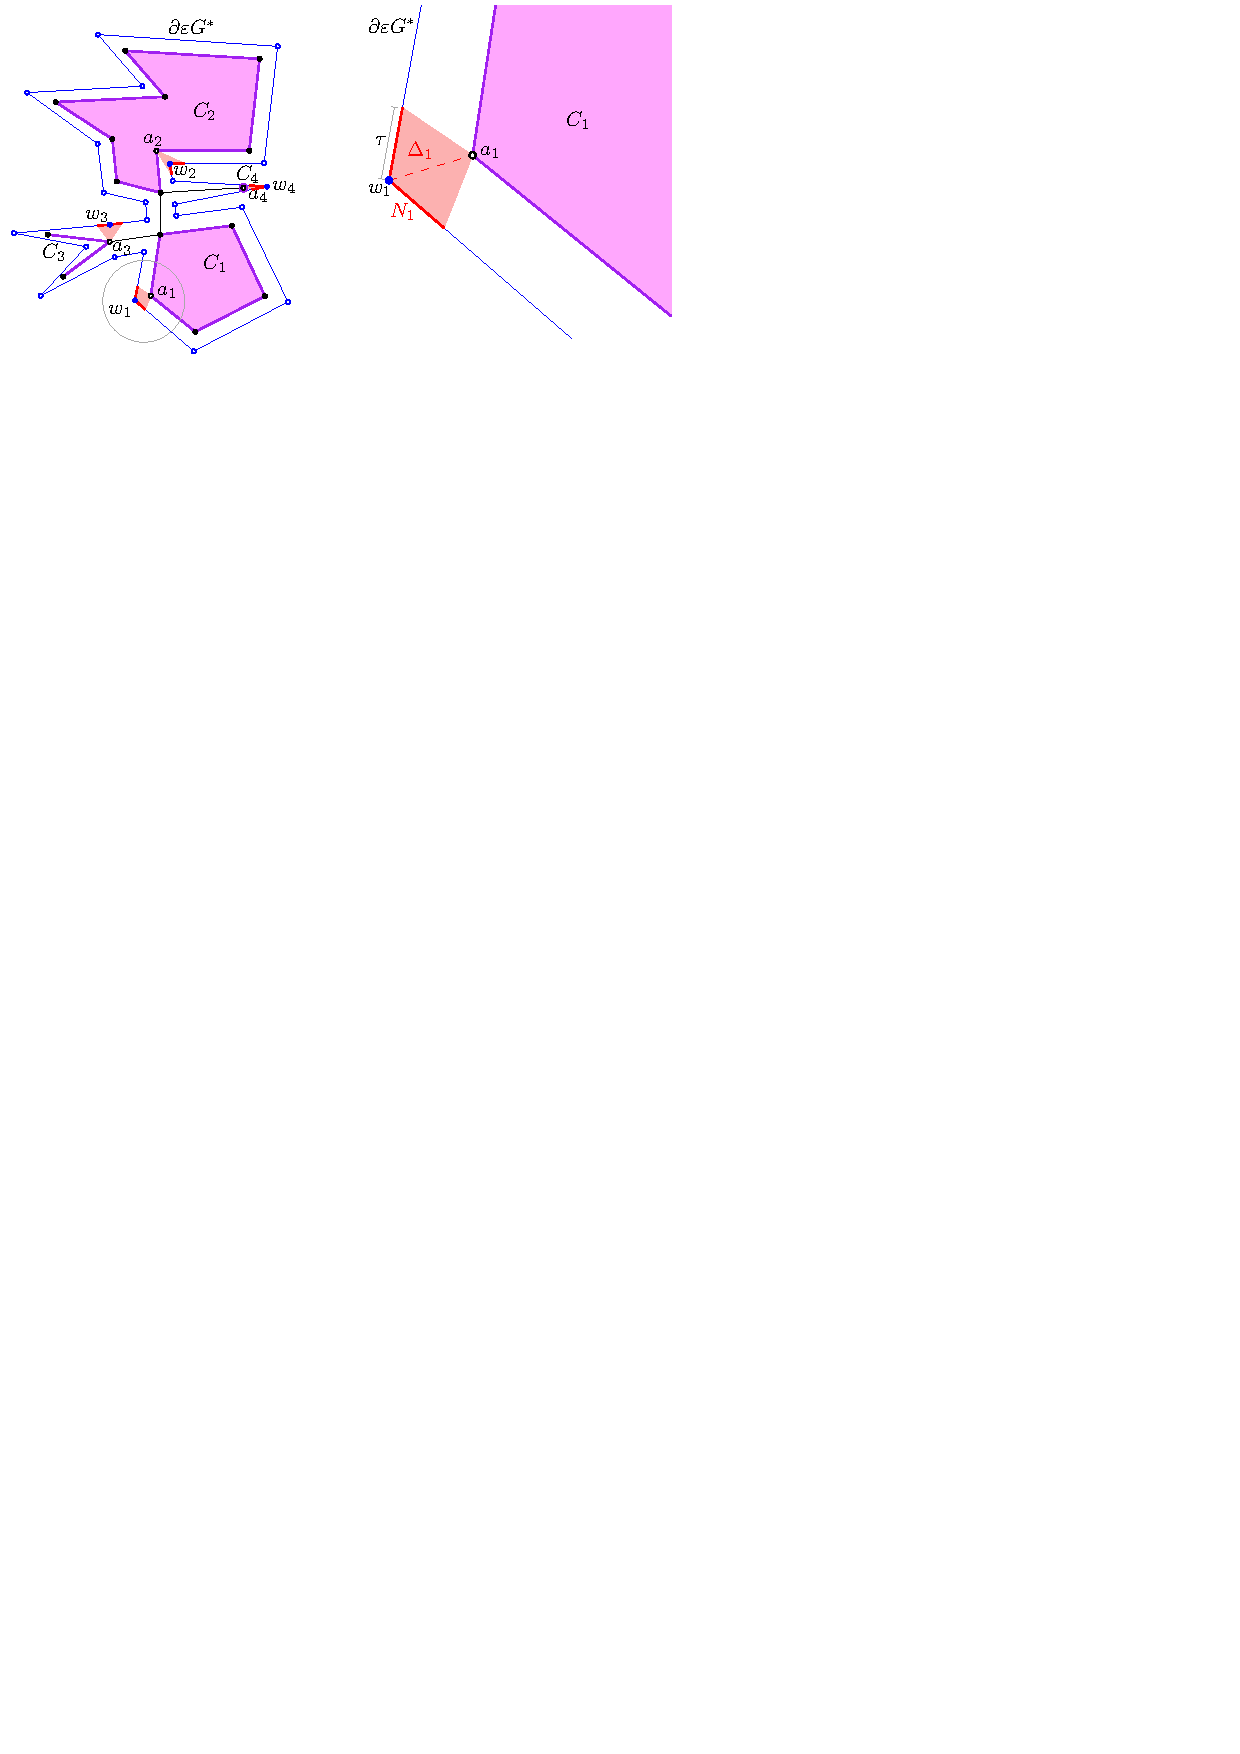
\includegraphics{img/Neighborhood.pdf}
%[width=1\textwidth]
\caption{\small }
\label{fig:Neighborhood}
\end{figure}

Assume that we have constructed a path $R$ that connects $a_1$ with $a_j$ for some $1\leq j\leq r$ (initially $j = 1$).
Moreover, assume that the escape invariant holds.
To extend $R$, we create a new path that connects $a_j$ with $a_{j+1}$ without crossing $R$ while maintaining the invariant. 
Recall that we consider $\partial_\varepsilon G_i^*$ to be a path with both endpoints on $w_1$.


If $j>1$, then we need to be careful in our way out of $a_j$ as we want $R$ to leave $C_j$ to its right. 
If the path $R$ together with the edge $a_j w_j$ leaves $C_j$ to its right, then walk from $a_j$ to $w_j$ in straight line.
Because the escape invariant holds, we know that $w_j$ is $R$-visible form $a_i$ and hence, this edge does not cross $R$.
If $R$ together with $a_j w_j$ does not leave $C_j$ to its right, then walk from $a_j$ to $\partial_\lambda C_j$ instead and traverse $\partial_\lambda C_j$ in clockwise order without crossing $R$ before moving to $w_j$ on $\partial_\varepsilon G^*$. In this way, we guarantee that $C_j$ lies to the right of the constructed path; see Figure~\ref{fig: Component to the right} for an illustration. 
Because $\lambda < \delta < \varepsilon$ and since $a_i\in V(R)$, the escape invariant is preserved.

\begin{figure}[tb]
\centering
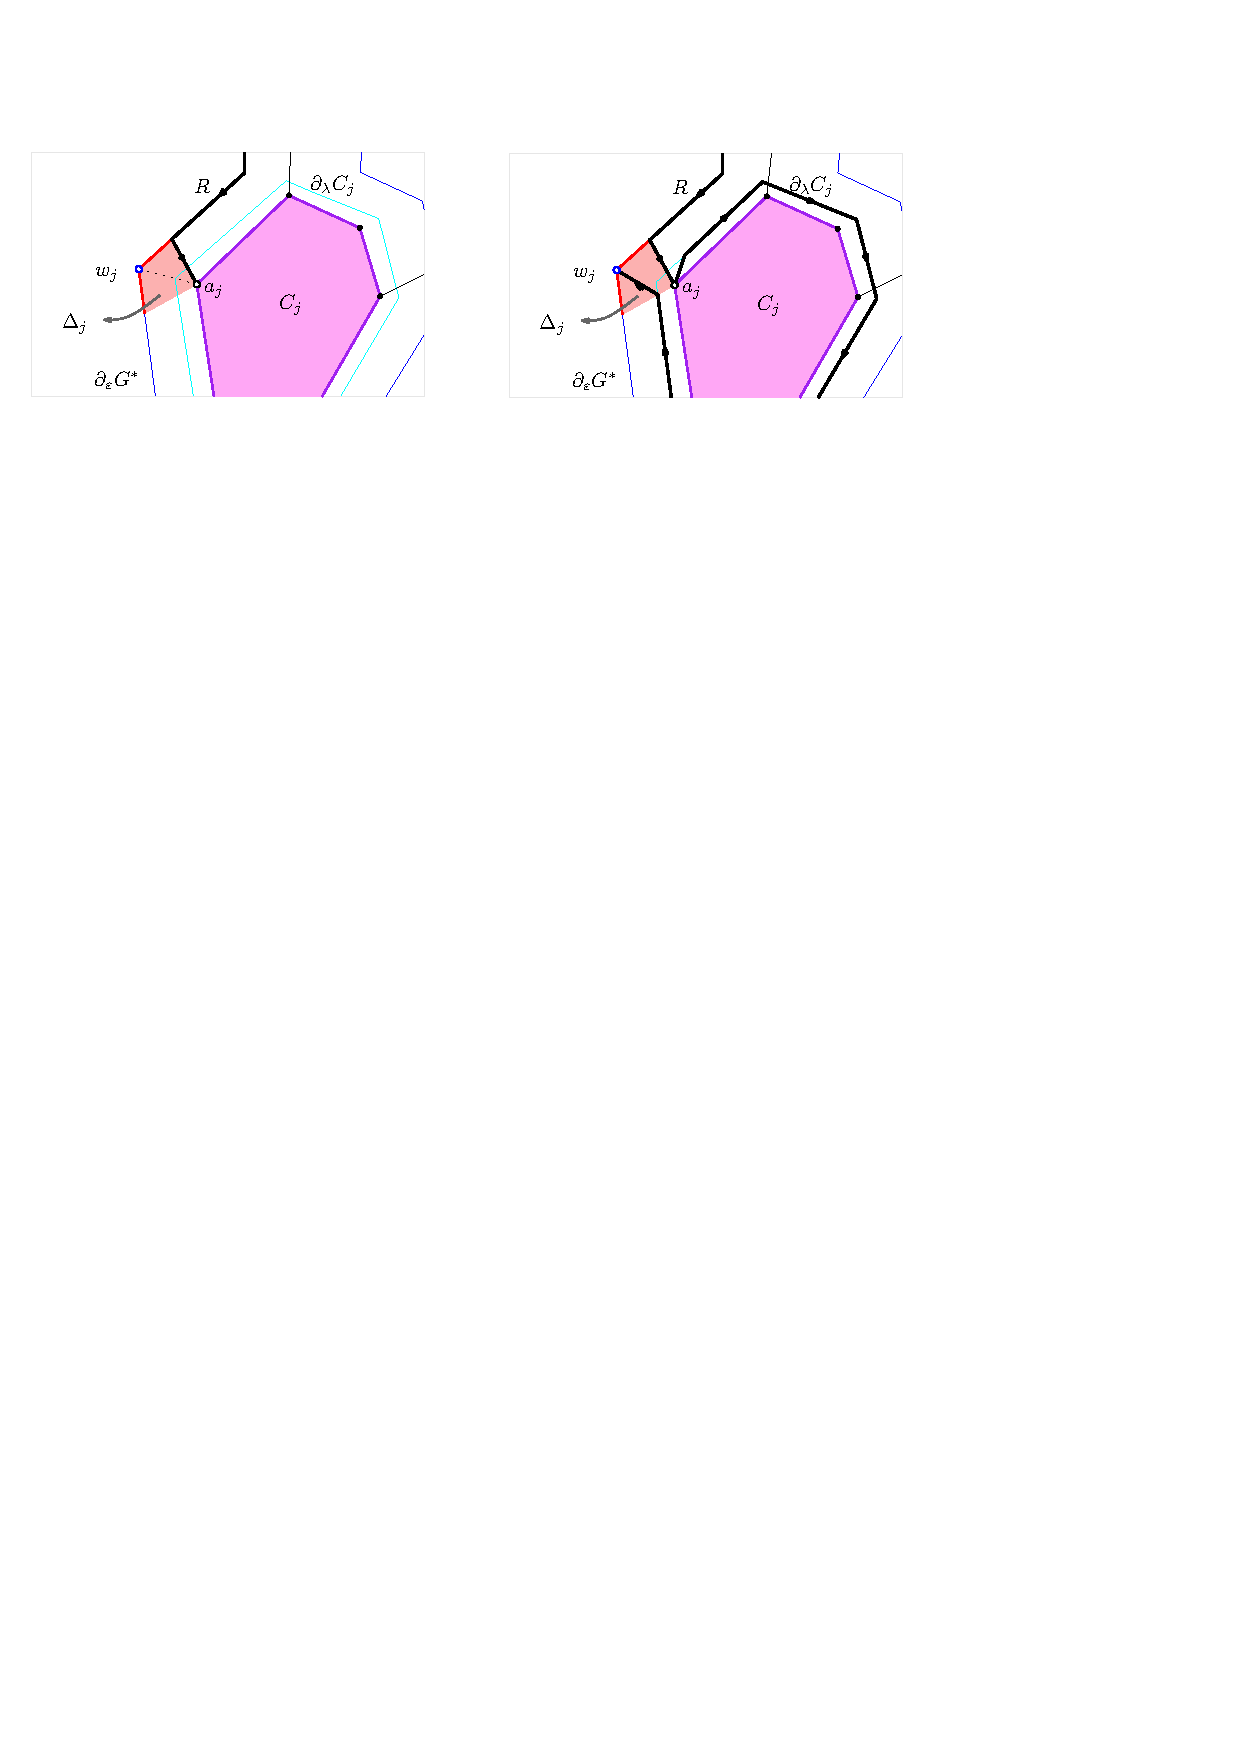
\includegraphics[width=1\textwidth]{img/ComponentToTheRight.pdf}
\caption{\small }
\label{fig: Component to the right}
\end{figure}

After reaching $w_j$, we follow $\partial_\varepsilon G^*$ along the shortest walk that connects $w_j$ with $w_{j+1}$. 
However, whenever we reach an endpoint of $N_i$ for some $1\leq i\leq r$ such that $a_i\notin V(R)$, we take a detour to the other endpoint of $N_i$ while avoiding its interior. 
In this way, the points in the interior of $N_i$ remain $R$-visible from $a_i$ (including $w_i$). Formally, we walk from the reached endpoint of $N_i$ to $\partial_\delta C_i\setminus \Delta_i$ along the boundary of $\Delta_i$. Then, we traverse the path $\partial_\delta C_i\setminus \Delta_i$ before moving to the other endpoint of $N_i$ from the endpoint of $\partial_\delta C_i \setminus \Delta_i$. In this way, we avoid crossing the cone $\Delta_i$; see Figure~\ref{fig:Skip Component} for an illustration. 
Note that $R$ does not intersect the interior of the simple polygon bounded by $\partial_\delta C_i$ nor the interior of $\Delta_i$.
Moreover, $R$ never goes out of the simple polygon bounded by $\partial_\varepsilon G^*$.

\begin{figure}[tb]
\centering
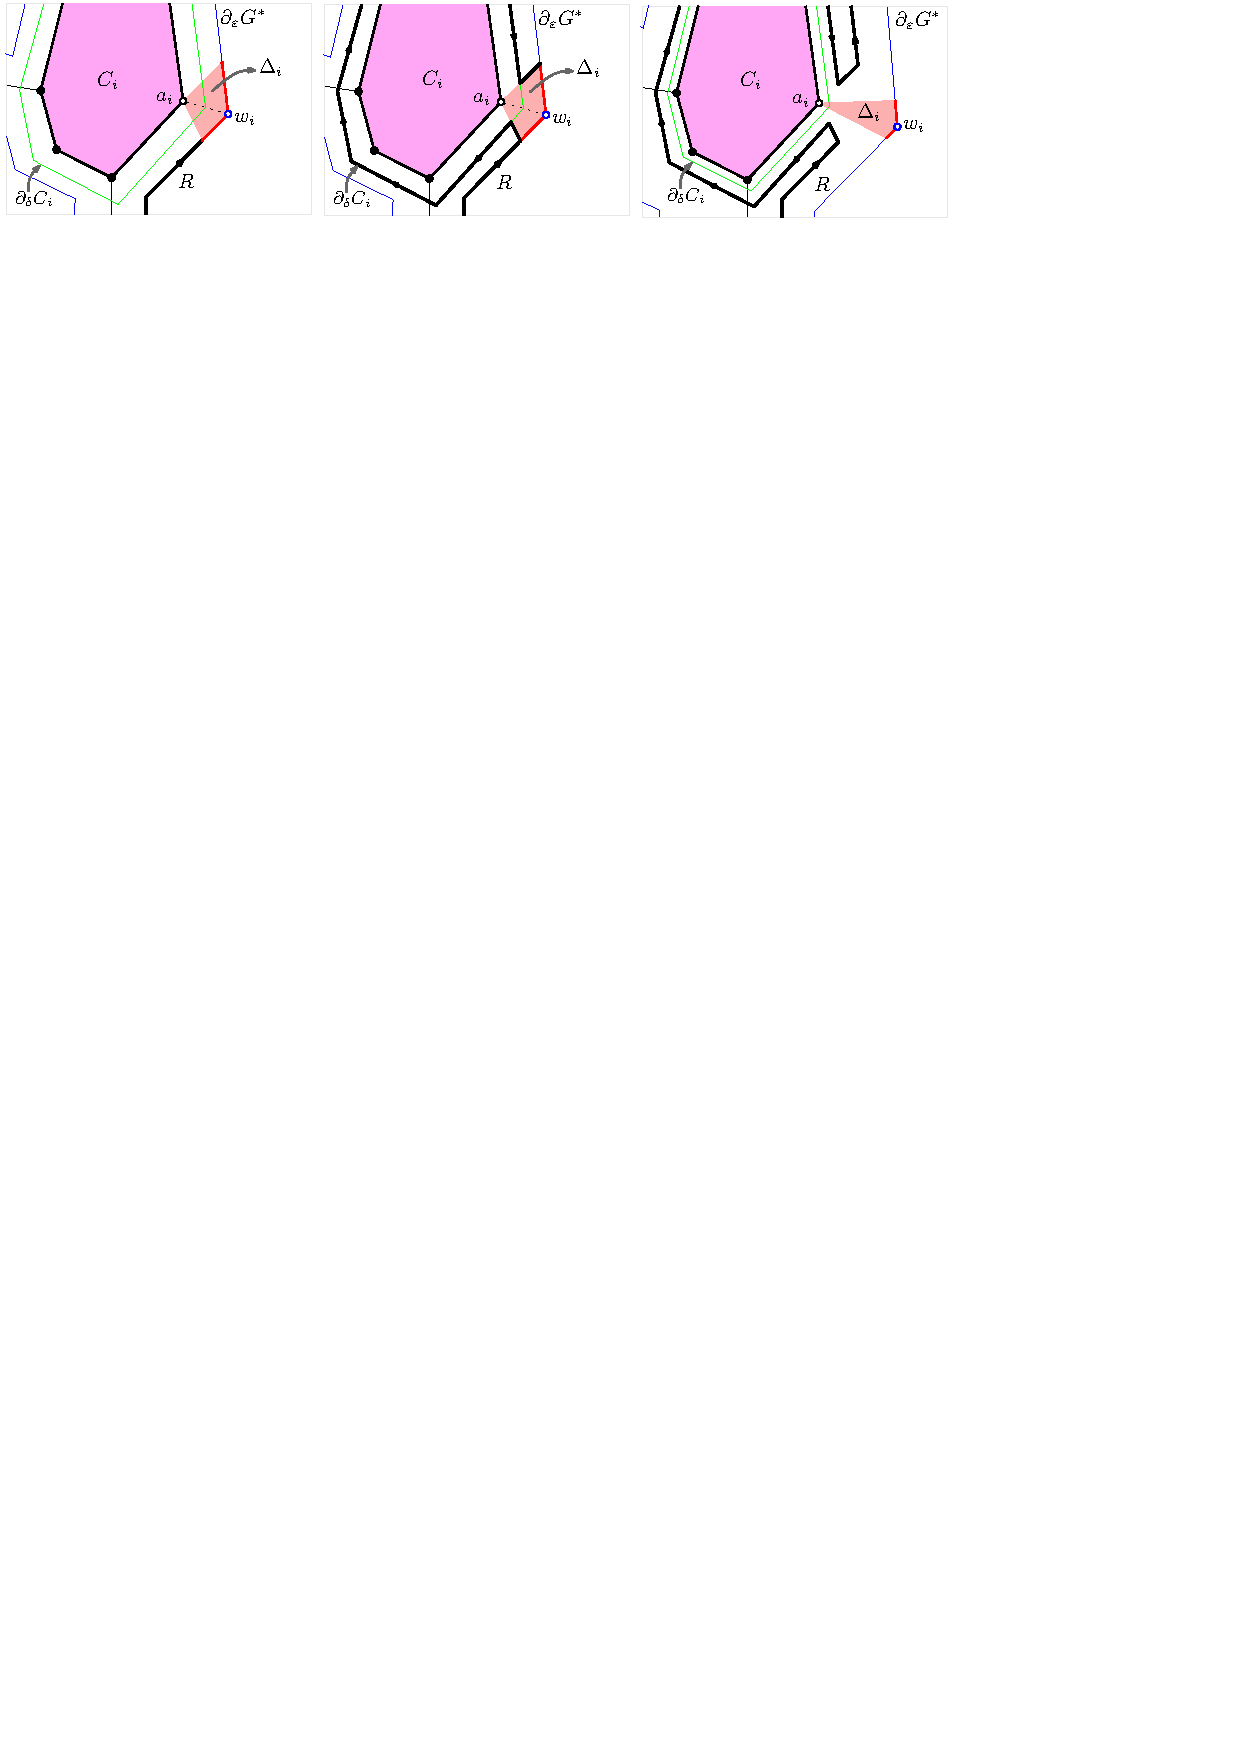
\includegraphics[width=1\textwidth]{img/SkipComponent.pdf}
\caption{\small }
\label{fig:Skip Component}
\end{figure}

Once we go around $C_i$, we are back on $\partial_\varepsilon G^*$ on the other endpoint of $N_i$. In this way, we continue going towards~$w_{j+1}$ along $\partial_\varepsilon G^*$ until reaching an endpoint of $N_{j+1}$.
Once we reach an endpoint of $N_{j+1}$, we move directly from this endpoint to $a_{j+1}$.

Because $\partial_\varepsilon G^*$ is isomorphic to $\varphi$, the constructed $a_j$-$a_{j+1}$-path has length at most $|\varphi(a_j, a_{j+1})|$ plus the length of the boundaries of the components that we walked around. 
Because each avoided component has its attachment corner on the path $\varphi(a_j, a_{j+1})$, the length of the constructed $a_j$-$a_{j+1}$-path is $$O(|\varphi(a_j, a_{j+1})| + \sum_{a_i\in A(a_j, a_{j+1})} |C_i|) = O(\sigma_G(a_j, a_{j+1}))\ .$$

After reaching $a_{j+1}$, we increase $\varepsilon$ by a factor of two. Similarly, we decrease de value of $\delta$ by a factor of two. That is, after reaching $a_{j+1}$, $\varepsilon = \mu 2^{j+1}$ while $\delta = \mu/2^{j+1}$ and hence, we guarantee that $\lambda < \delta < \varepsilon$.
We can guarantee that $\partial_\varepsilon G^*$ remains simple, provided that the original choice of $\mu$ is sufficiently small. 
Finally, for each $1\leq i\leq n$, we reduce the size of the neighborhood $N_i$ by reducing $\tau$ by a factor of two and updating the cone $\Delta_i$ accordingly, i.e., we narrow the cone $\Delta_i$; see Figure~\ref{fig:Skip Component} (c). 

Recall that for each $a_i\notin R$, $R$ intersected neither the interior of $\Delta_i$ nor the interior of the polygon bounded by $\partial_\delta C_i$. Moreover, $R$ never went out of $\partial_\varepsilon G^*$.
Therefore, after increasing (\emph{resp.} reducing) $\varepsilon$ (\emph{resp.} $\delta$), we preserve the correctness invariant should there be a subsequent round of the algorithm.
We repeat this algorithm until all attachment corners of $G$ are visited by $R$.

\begin{lemma}\label{lemma:Path for connected augmentations}
Given an arbitrary order $a_1, \ldots, a_r$ of the attachment corners of $G$, the previous algorithm computes a path $R$ connecting all attachment corners of $G$ in the given order such that $R\cup G$ is plane, $|R| = O(\sum_{j=1}^{n-1} \sigma_G(a_j, a_{j+1}))$, and for each $1\leq i\leq r$, $C_i$ lies to the right of $R$ when oriented from $a_1$ to $a_r$.
\end{lemma}
\begin{proof}
By construction, the attachment corners are visited by $R$ in the given order. For each component $C_i$, $a_i$ is the only vertex of $C_i$ visited by $R$. Moreover, the construction guarantees that $C_i$ lies to the right of $R$ when oriented from $a_1$ to $a_r$.

To prove that $R$ is plane, recall that in each round we extend $R$ by constructing  a path $\gamma_j$ that connects $a_j$ with $a_{j+1}$. We claim that at this point, no edge of $\gamma_j$ crosses the portion of $R$ constructed so far.
Indeed, because the value of $\varepsilon$ (\emph{resp.} $\delta$) increases (\emph{resp.} decreases) by a factor of two in each round, the edges of $\gamma_j$ that lie on the boundaries of some $\partial_\delta C_i$ or on $\partial_\varepsilon G^*$ cannot cross $R$ by the escape invariant.
Moreover, this invariant states that for each $a_i\notin R$, $R$ does not intersect~$\Delta_i$.
Because each cone $\Delta_i$ is narrowed in each round, the edges of $\gamma_j$ that lie on the boundary of this cone cannot cross $R$. Finally, because $\lambda < \delta$, the edges of $\gamma_j$ that lie on $\partial_\lambda C_j$ do not cross $R$. Therefore, we conclude that by concatenating $\gamma_j$ and $R$, we obtain a plane path.

Because the length of $\gamma_j$ is $O(\sigma_G(a_j, a_{j+1}))$, the total length of $R$ after connecting every attachment corner is given by $|R| = O(\sum_{j=1}^{n-1} \sigma_G(a_j, a_{j+1}))$.
\end{proof}

\subsection{Compatible drawings of planar graphs}
Let $\mathcal G$ be a planar graph with $n$ vertices and $r$ connected components.
Let $G_1, \ldots, G_k$ be $k$ plane isomorphic drawings of $\mathcal G$. 
We show how to construct a compatible augmentation of $\mathcal G$ of size $O(nr^{1-1/k})$.

Let $C_1, \ldots, C_r$ be the connected components of $\mathcal G$.
Because all the plane drawings of $\mathcal G$ that we consider are isomorphic, the boundaries of corresponding components in different drawings are also isomorphic. Thus, for each $1\leq j\leq r$, we can choose an attachment corner $a_j$ in $\partial C_j$ such that $a_j$ is adjacent to the outer face. Note that this corner has isomorphic copies in each of the embeddings of $G$.

For each $1\leq j\leq r$, let $G_j^*$ be a connected augmentation of $G_j$ (see Section~\ref{section: connected augmentations} for the construction of such a graph).
For each $1\leq i\leq k$ and for each $1\leq j\leq r$, let $rank_i(j) = \sigma_{G_i}(a_1, a_j)$.
For each $1\leq j\leq r$, we define a point $x_j\in \mathbb{R}^k$ that correspond to the component $C_j$ such that 
$x_j = (rank_1(a_j), rank_2(a_j), \ldots, rank_k(a_j))$. Let $X = \{x_1, \ldots, x_r\}$ be a set of points in $\mathbb{R}^k$. 
Note that Lemma~\ref{lemma:Contained in integer grid} implies that $X$ is contained in an integer grid of side length $5n$ of dimension~$k$.

Let $P$ be the shortest hamiltonian path of $X$, i.e., the shortest path that visits every point of $X$.
Because $X$ is contained in the $k$-dimensional integer grid of side-length $5n$ and from the fact that $|X| = r$, we known that the length of $P$ is $O(nr^{1-1/k})$~\cite{}.

Note that the order of the points of $P$ induces an order on the components of $\mathcal G$ and hence, an order on the attachment corners of each $G_i$. 

\begin{theorem}
For each $1\leq i\leq k$, we can construct a path $R_i$ of length $O(nr^{1-1/k})$ that connects every component of $G_i$ such that $G_i\cup R_i$ is plane. Moreover, for each $1\leq i<j\leq k$, $G_i\cup R_i$ is isomorphic to $G_j\cup R_j$.
\end{theorem}
\begin{proof}
For each $G_i$, we use Lemma~\ref{lemma:Path for connected augmentations} to construct a plane path $R_i$ that connects the attachment corners of $G_i$ in the order induced by $P$.
Assume that $(a_1, \ldots, a_r)$ is the order of the attachment corners of $G_i$ induced by $P$.
Lemma~\ref{lemma:Path for connected augmentations} implies that $|R_i| = O(\sum_{j=1}^{n-1} \sigma_{G_i}(a_j, a_{j+1}))$.

Because $\sigma_{G_i}(a_j, a_{j+1}) = |\sigma_{G_i}(a_1, a_{j+1}) - \sigma_{G_i}(a_1, a_j)|$ by Lemma~\ref{lemma:Contained in integer grid} and from the fact that $rank_i(j) = \sigma_{G_i}(a_1, a_j)$, we get that  $\sigma_{G_i}(a_j, a_{j+1}) = |rank_i(j+1) - rank_i(j)|$.
Therefore, $|R_i|  = O\left(\sum_{j=1}^{n-1} |rank_i(j+1) - rank_i(j)|\right)$.

Let $d_j$ denote the distance between $x_j$ and $x_{j+1}$ in $P$. 
Because $|rank_i(j+1) - rank_i(j)|$ represents the difference in the $i$-th coordinates of $x_j$ and $x_{j+1}$, by the triangle inequality we infer that $|rank_i(j+1) - rank_i(j)| \leq  d_j$ . 
Therefore, the path contained in $R_i$ has length $O\left(\sum_{j=1}^{n-1} |rank_i(j+1) - rank_i(j)|\right) = O(\sum_{j=1}^{n-1} d_j)$. 
Because $\sum_{j=1}^{n-1} d_j = |P| = O(nr^{1-1/k})$, the length $R_i$ is $O(nr^{1-1/k})$.

Since each $R_i$ visits each component only at its attachment corner and from the fact that $R_i$ leaves every component to the right when oriented from $a_1$ to $a_r$, we conclude that $G_i\cup R_i$ is isomorphic to $G_j\cup R_j$ for each $1\leq i<j\leq k$.
\end{proof}

\section{Lower Bounds}

Our lower bounds are based on the following lemma. In words, this lemma says that we can find $k$ permutations of $\{1,\ldots,r\}$ such that, for half the indices $i\in\{1,\ldots,r\}$, and every $j\in\{1,\ldots,r\}\setminus\{i\}$, there is a permutation in which $i$ and $j$ are at distance $\Omega(r^{1-1/k})$.

\begin{lemma}\label{lem:permutations}
Let $t=(1/2)^{1+1/k}\cdot(r-1)^{1-1/k}$.  There exists permutations $\pi^{(1)},\ldots,\pi^{(k)}$ of $\{1,\ldots,r\}$ such that, for at least half the values of $i\in\{1,\ldots,r\}$ and for every $j\in\{1,\ldots,r\}\setminus\{i\}$, 
\begin{equation}
 \max\left\{\left|\pi^{(s)}_i-\pi^{(s)}_j\right|\colon s\in\{1,\ldots,k\} \right\}
 \ge t \enspace .
     \label{eq:perm}
\end{equation}
\end{lemma}

\begin{proof}
  This proof is an application of the probabilistic method.  Select each
  of $\pi^{(1)},\ldots,\pi^{(k)}$ independently and uniformly from among
  all $r!$ permutations of $\{1,\ldots,r\}$.  Fix a particular index $i$
  and a particular index $j$.  For a particular $s\in\{1,\ldots,k\}$, the
  probability that $|\pi^{(s)}_i-\pi^{(s)}_j|\le t$ is at most $2t/(r-1)$
  since the set
  $\{\hat \jmath\in\{1,\ldots,r\} \colon |\pi^{(s)}_i-\pi^{(s)}_{\hat
   \jmath}|\le t\}$ is a random subset of $2t$ elements drawn without
  replacement from $\{1,\ldots,r\}\setminus \{i\}$.

  Therefore, since $\pi^{(1)},\ldots,\pi^{(k)}$ are chosen independently, 
  \[
    \Pr\left\{\max\left\{\left|\pi^{(s)}_i-\pi^{(s)}_j\right|\colon s\in\{1,\ldots,k\} \right\}\le t\right\} \le (2t/(r-1))^k = \frac{1}{2(r-1)} \enspace .
  \]
  In particular, the expected number of such
  $j\in\{1,\ldots,r\}\setminus\{i\}$ is at most $1/2$ so, by Markov's
  Inequality, the probability that there exists at least one such $j$
  is at most $1/2$.  Thus, with probability at least $1/2$, the index $i$
  satisfies \eqref{eq:perm} and therefore the expected number of indices $i\in\{1,\ldots,r\}$
  that satisfy \eqref{eq:perm} is $r/2$.  We conclude that there must exist
  some permutations $\pi^{(1)},\ldots,\pi^{(k)}$ that satisfy \eqref{eq:perm}
  for at least half the indices $i\in\{1,\ldots,r\}$.
\end{proof}

Using Lemma~\ref{lem:permutations}, we can prove a lower bound that matches the upper bound obtained in our general construction.

\begin{theorem}\label{thm:lower-bound}
  For every integer $n$ and every $r\in\{1,\ldots,\lfloor n/4\rfloor\}$,
  there exists a graph $\mathcal G$ having $n$ vertices, $r$ connected
  components, and $k$ isomorphic drawings $G_1,\ldots,G_k$ such that
  any compatible augmentation of $G$ has size $\Omega(nr^{1-1/k})$.
\end{theorem}

\begin{proof}
Since the lemma only claims an asymptotic result, we may assume without
loss of generality that $r$ is even and that $2r$ divides $n$.

The graph $\mathcal G$ consists of $r$ disjoint paths,
$\mathcal{C}_1,\ldots,\mathcal{C}_r$, each of length $n/r$.  Each of the
drawings $G_1$,\ldots,$G_k$ embeds the vertices of $\mathcal G$ on the
same point and segment set. The point set consists of the vertices of
$r$ nested regular $n/r$-gons, $P_1,\ldots,P_r$, each centered at the
origin and having nearly the same size. Refer to Figure~\ref{fig:lower-bound}.a. More precisely, $P_1\subset
P_2\subset\cdots\subset P_r$ and the sizes are chosen so that any segment
joining two non-consecutive vertices of $P_i$ intersects the interior
of $P_{i-1}$.

\begin{figure}
  \begin{center}
  \begin{tabular}{cc}
    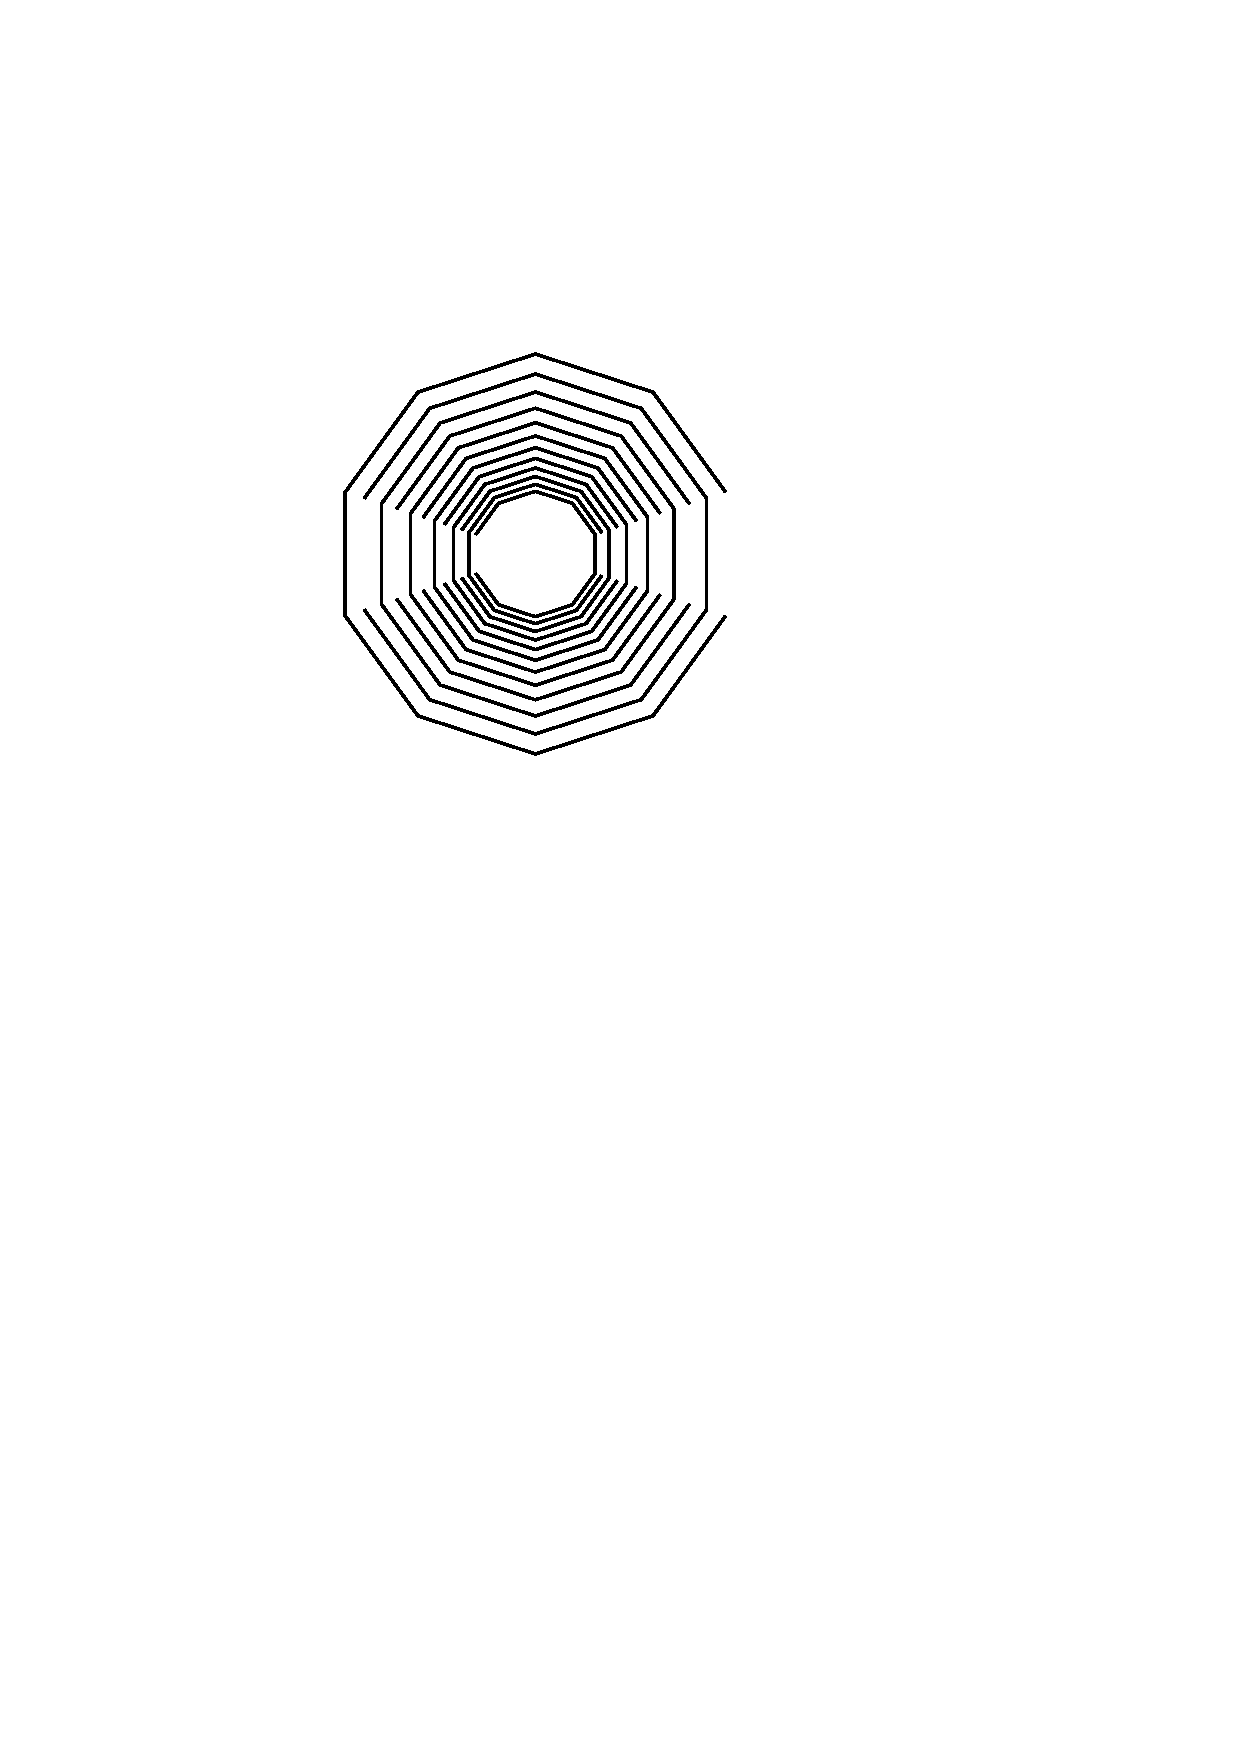
\includegraphics{img/lower-bound-1} &
    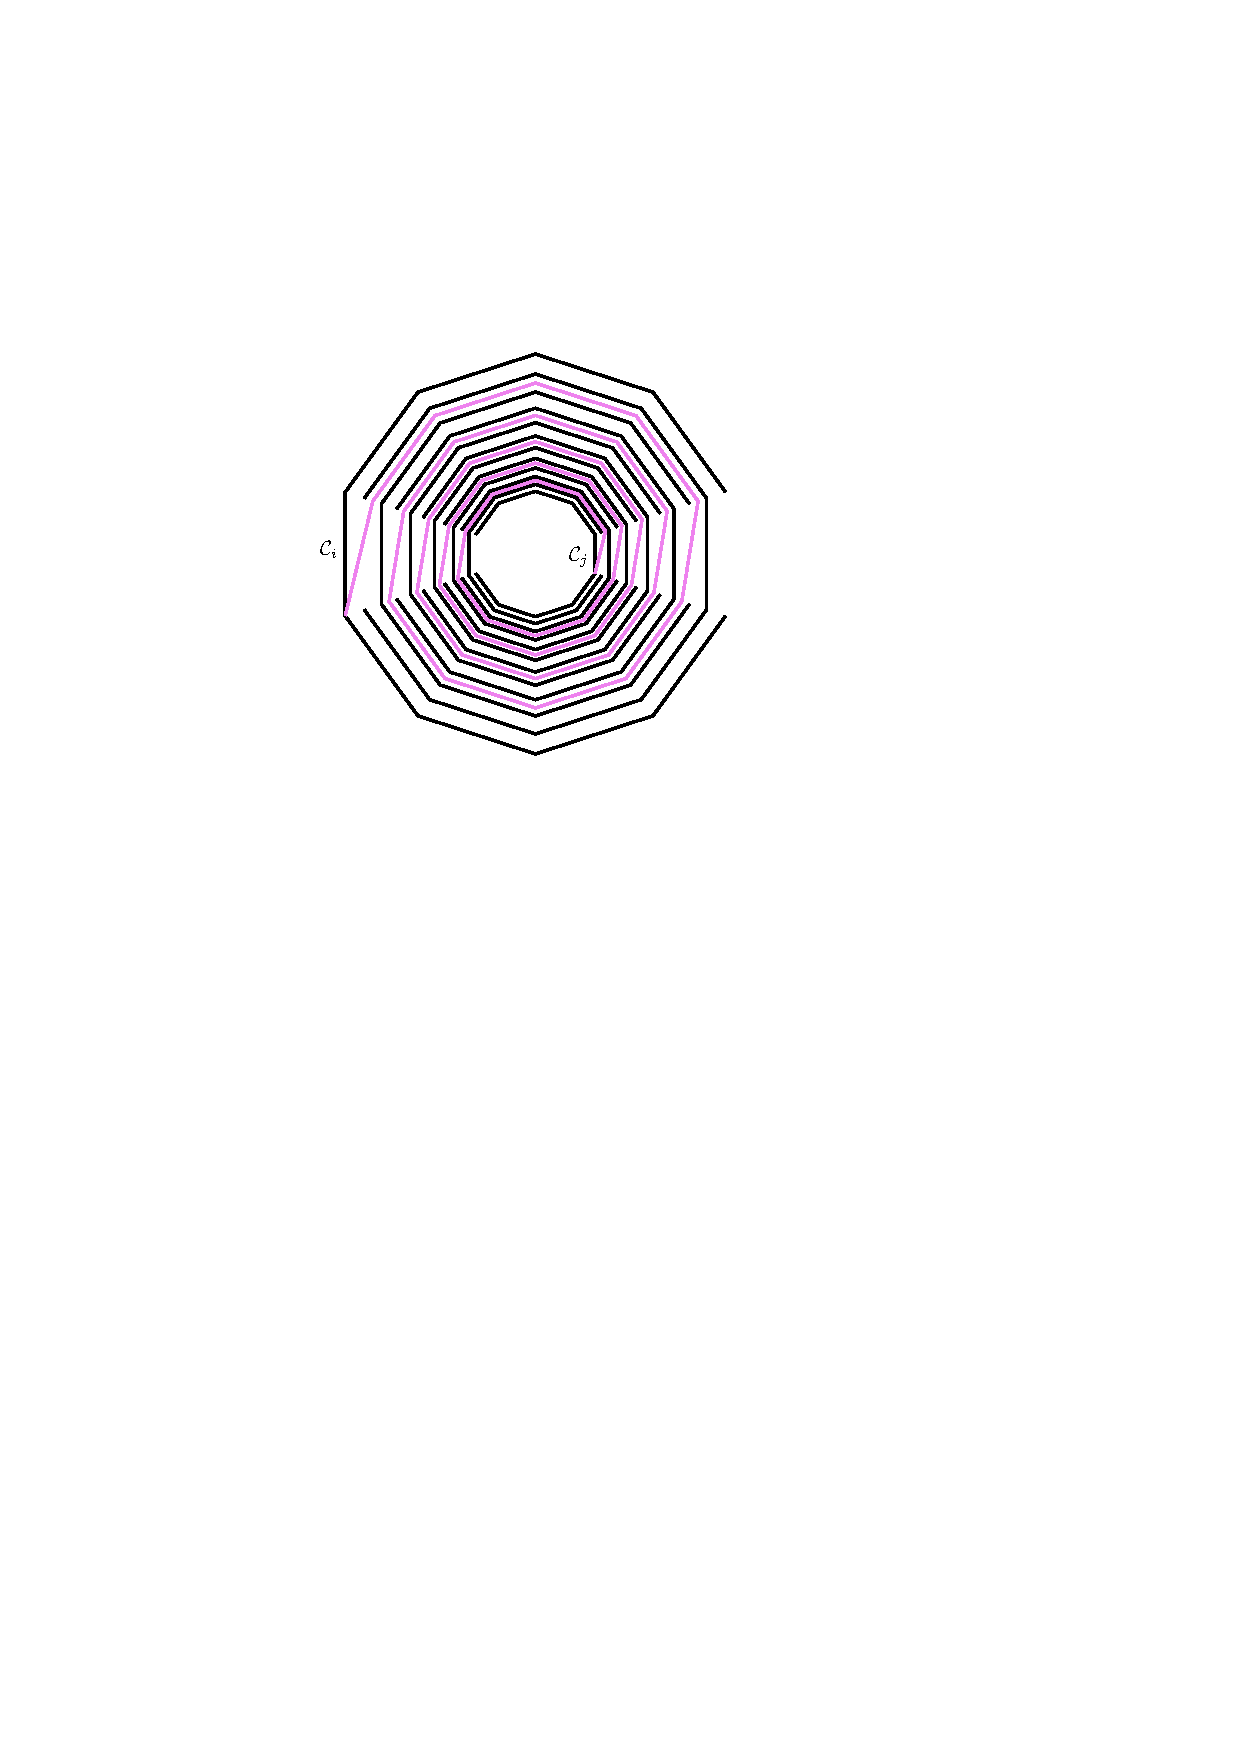
\includegraphics{img/lower-bound-2} \\
    (a) & (b)
  \end{tabular}
  \end{center}
  \caption{In the lower bound of Theorem~\ref{thm:lower-bound}, (a)~all
    drawings use the same set of points for vertices and segments for
    edges and (b)~the drawing of a path that joins $\mathcal{C}_i$ to
    $\mathcal{C}_j$ must travel around all the paths embedded between the
    drawing of $\mathcal{C}_i$ and the drawing of $\mathcal{C}_j$.}
  \label{fig:lower-bound}
\end{figure}

The drawings $G_1,\ldots,G_k$ are obtained from the permutations
$\pi^{(1)},\ldots,\pi^{(k)}$ given by Lemma~\ref{lem:permutations}.
In the drawing $G_x$, the path $\mathcal C_i$ is embedded on the vertices
of $P_{\pi^{(x)}_i}$. If $y=\pi^{(x)}_i$ is even, the drawing uses
all the edges of $P_y$ except the left-most edge.  If $y$ is odd, the
drawing uses all the edges of $P_y$ except the right-most edge.

Now, without loss of generality, consider some edge-minimal compatible
augmentation $\mathcal H$ of $\mathcal G$.  For each component
$\mathcal{C}_i$ of $G$, let $T_i$ be any path in $\mathcal H$ that has
one endpoint on $\mathcal C_i$, one endpoint on some other component
$\mathcal{C}_j$, $j\neq i$, and no vertices of $\mathcal G$ in its
interior.

Now, for each of the $r/2$ indices $i\in\{1,\ldots,r\}$ that satisfy
\eqref{eq:perm}, the path $T_i$ joins a vertex of
$P_{\pi^{(s)}_i}$ to a vertex of $P_{\pi^{(s)}_j}$, $j\neq
i$, and $|\pi^{(s)}_i-\pi^{(s)}_i|\ge t$.  This path must
have length $\Omega(tn/r)$ since it has to ``go around'' the
paths between $P_{\pi^{(s)}_i}$ and $P_{\pi^{(s)}_j}$; see
Figure~\ref{fig:lower-bound}.b.

Thus far, we have shown that for at least $r/2$ values of
$i\in\{1,\ldots,r\}$, the component $C_i$ is the endpoint of a
path, $T_i$, of length at least $\Omega(tn/r)=\Omega(nr^{-1/k})$.
It is tempting to claim the result at this point, since
$(r/2)\cdot\Omega(nr^{-1/k})=\Omega(nr^{1-1/k})$. Unfortunately, there
is a little more work that needs to be done, since two such paths $T_i$
and $T_j$ may not be disjoint, so summing their lengths double-counts
the contribution of the shared portion.

To finish up we note that, since the augmentation $\mathcal{H}$ is minimal,
it is a tree; $\mathcal G$ contains no cycles, so any cycle in $\mathcal H$ contains an edge not in $\mathcal G$ that could be removed.  Now, observe that if we traverse the outer face of (any planar drawing of) $\mathcal H$ then we obtain a non-simple path, $P$, that traverses each edge of $\mathcal{H}$ exactly twice. If we consider the set of maximal subpaths of $P$ with no vertex of $\mathcal G$ in their interior, we obtain a set of $r$ paths, $Q_1,\ldots,Q_{r}$ and, for every component $\mathcal C_i$ of $\mathcal G$, there is a vertex of $\mathcal C_i$ that is an endpoint of at least one such path.  Therefore, from the preceding discussion, the total length of $Q_1\ldots,Q_{r}$ is $\Omega(nr^{1-1/k})$.  But since each edge of $\mathcal H$ appears at most twice in these subpaths, we conclude that $\mathcal H$ has $\Omega(nr^{1-1/k})$ edges.  Since $\mathcal H$ is a tree, it has $\Omega(nr^{1-1/k})$ vertices.
\end{proof}


\bibliographystyle{plain}
\bibliography{tmp}















\end{document}  
